
\chapter{Gráfok}\label{chap:grafok}
\section{Alapfogalmak}\label{sec:graf_alapok}
\begin{description}
{\large\item [{Szerző:}] Csurka-Molnár Hanna (Didaktikai mesteri -- Matematika, II.
év) }
\end{description}
\begin{definition}[Gráf]{def:graf}
A gráf csúcsokból és élekből álló halmaz, ahol az élek csúcsokat
kötnek össze, és minden élre legalább egy, legfeljebb két csúcs illeszkedik.
\end{definition}

\begin{definition}[Gráf rendje]{def:graf_rendje}
    A gráf rendjén a csúcsok számát értjük.
\end{definition}

\begin{definition}[Gráf nagysága]{def:graf_nagysaga}
    A gráf nagyságán az élek számát értjük.
\end{definition}

\begin{definition}[Párhuzamos élek]{def:parhuzamos_elek}
    Ha két csúcsot egynél több él köt össze, akkor azokat párhuzamos éleknek nevezzük.
\end{definition}

\begin{definition}[Hurokél]{def:hurokel}
    Ha egy élre egy csúcs illeszkedik, azaz egy él két végpontja azonos, akkor azt az élet hurokélnek nevezzük.
\end{definition}

\begin{definition}[Fokszám]{def:fokszam}
    Egy csúcshoz illeszkedő élek számát fokszámnak nevezzük
\end{definition}
\vspace*{1cm}
\begin{definition}[Izolált csúcs]{def:izolalt_csucs}
    Izolált csúcs, ha nem kötődik hozzá él.
\end{definition}

\begin{definition}[Levél]{def:level}
    Levél, ha egy él kötődik hozzá.
\end{definition}

\begin{theorem}{thm:fokszamcsucsok}
    Minden gráfban a csúcsok fokszámának összege az élek számának kétszerese.
\end{theorem}

\begin{proof}
    Egy csúcs fokszáma alatt az élcsatlakozásainak a számát értjük.
    Egy hurokél kétszer csatlakozik egy csúcshoz, így annak fokszámát kettővel növeli.
    Egy nem hurok él két csúcshoz csatlakozik, azok fokszámát $1-1$-el növelve.
    Így minden él a gráf csúcsainak összfokszámát $2$-vel növeli, vagyis a fokszámok összege $2M$, ahol $M$ az élek száma a gráfban.
\end{proof}

\begin{definition}[Egyszerű gráf]{def:egyszeru_graf}
    Ha egy gráfban nincsenek párhuzamos élek és nincs hurokél sem, akkor az egy egyszerű gráf. 
\end{definition}

\begin{definition}[Teljes gráf]{def:teljes_graf}
    Ha egy gráfnak minden csúcsából pontosan egy él vezet a gráf összes többi csúcsához, akkor az teljes gráf. 
\end{definition}

\begin{theorem}{thm:teljes_graf_n}
    Az n csúcsú teljes gráf éleinek a száma: $\frac{N \cdot (N-1)}{2}$.
\end{theorem}

\begin{proof}
    Egy teljes gráf minden csúcsából minden csúcsába megy él.
    Egy csúcsból $N-1$ csúcsba tudunk élet húzni.
    Azonban, ha minden csúcsból megszámoljuk az $N-1$ élet, akkor $N(N-1)$-et kapunk, viszont minden élet kétszer számoltunk, mert az élek irányítatlanok.
    Tehát az élek száma $\frac{N \cdot (N-1)}{2}$.

    Másként az éleket száma úgy adható meg, hogy hány féle módon tudunk a gráf csúcsaiból $2$-t kiválasztani és azokat összekötni?
    Ezt a ${N\choose2} =\frac{N(N-1)}{2}$ adja meg.
\end{proof}

\begin{definition}[Gráf komplementere]{def:komplementer_graf}
    Ha két egyszerű gráf csúcsai ugyanazok, de az egyik gráfban pontosan azokat a csúcsokat kötöttük össze, amiket a másikban nem, akkor az mondjuk, hogy a két gráf egymás komplementere
\end{definition}

\begin{definition}[Irányított gráf]{def:iranyitott_graf}
    Irányított gráfnak nevezzük a csúcsokból és csúcspárokat összekötő irányított vonalakból álló alakzatokat. Ennek éleit irányított éleknek nevezzük.
\end{definition}

\begin{definition}[Részgráf]{def:reszgraf}
    Egy gráf részgráfja minden olyan gráf, amelyet úgy kaphatunk, hogy az eredeti gráf élei és csúcsai közül bizonyosakat elhagyunk.
\end{definition}

\begin{definition}[Páros gráf]{def:paros_graf}
    Egy gráfot páros gráfnak nevezünk, ha csúcsai két diszjunkt részre – A és B – oszthatók úgy, hogy minden él egy A és egy B részben lévő csúcsot köt össze.
\end{definition}

\begin{definition}[Gráfizomorfizmus]{def:graf_izo}
    A gráfizomorfizmusok gráfok közötti bijektív struktúratartó leképezések, értve ezalatt azt, hogy a függvény és az inverz függvény egyaránt szomszédos csúcsokat szomszédos csúcsokra képez le. Az általuk meghatározott ekvivalenciarelációt gráfizomorfiának nevezzük.
\end{definition}

\begin{definition}[Séta]{def:seta}
    Sétának nevezzük a gráf éleinek egymáshoz csatlakozó sorozatát, amelyben ugyanazok az élek és csúcsok többször is előfordulhatnak.
\end{definition}

\begin{definition}[Vonal]{def:vonal}
    Vonalnak nevezzük a gráf egymáshoz csatlakozó éleinek olyan sorát, amelyben egyetlen él sem szerepel egynél többször.
\end{definition}

\begin{definition}[Út]{def:ut}
    Útnak nevezzük a gráf egymáshoz csatlakozó éleinek olyan sorát, amelyben egyetlen csúcson sem halad át egynél többször.
\end{definition}

\begin{definition}[Kör]{def:kor}
    Körnek nevezzük a kiinduló csúcsba visszavezető utat, azaz olyan élsorozatot, amely a kiinduló csúcsba tér vissza, valamint minden csúcs és minden él csak egyszer szerepel benne.
\end{definition}

\begin{definition}[Euler-vonal]{def:euler-vonal}
    A vonalak közül azokat, amelyekben a gráfnak minden éle szerepel, Euler-vonalnak nevezzük.
\end{definition}

\begin{definition}[Euler-kör]{def:euler-kor}
    A vonalak közül azokat, amelyeknek kezdő és végpontja azonos, és amelyekben a gráfnak minden éle szerepel, Euler-körnek nevezzük.
\end{definition}

\begin{theorem}{thm:euler-kor}
    Egy összefüggő gráfnak akkor és csak akkor van Euler-köre, ha a gráf minden csúcsának fokszáma páros szám.
\end{theorem}

\begin{proof}
    Először azt látjuk be, hogy ha a gráf tartalmaz Euler-kört, akkor minden csúcs foka páros.
    Ha elindulunk a gráf egyik csúcsából, és körbejárjuk az Euler-köre mentén, akkor minden csúcsba pontosan annyiszor megyünk be, ahányszor kimegyünk belőle.
    A bemenések és kimenések számának összege nyilvánvalóan páros, és ez egyben minden csúcsnál a fokszámot adja.
    
    Most azt bizonyítjuk, hogy ha minden csúcs foka páros, akkor valóban tartalmaz Euler-kört.
    Ezt a $G$ csúcsszámára vonatkozó teljes indukcióval bizonyítjuk.
    A legkisebb csúcsszámú olyan gráf, melynek minden fokszáma páros, a $N=3$ csúcsú teljes gráf, vagyis a háromszög.
    Ebben van Euler-kör.
    
    Tegyük fel, hogy minden $k<N$-ra igaz az állítás.
    Induljunk el $G$ egyik csúcsából, és haladjunk úgy az élek mentén, hogy egyiken sem megyünk át egynél többször.
    Ha elakadunk, vagyis az egyik csúcsból már nem vezet ki él, akkor az biztosan a kiindulási csúcs a fokszám páros volta miatt.
    Ekkor kaptunk egy zárt élsorozatot.
    Legyen $F$ egy olyan zárt élsorozat $G$-ben, melyben a lehető legtöbb él szerepel.
    
    A fenti eljárásban azért álltunk meg, mert a kezdőpontból nem indult ki újabb él, tehát az ebből a csúcsból kiinduló összes él $F$-ben van.
    Ha $F$ $G$-nek Euler-köre, akkor készen vagyunk.
    Amennyiben $F$ nem Euler-köre $G$-nek, akkor vizsgáljuk $G$-nek azt a részgráfját, mely pontosan azokat az éleket tartalmazza, amelyeket $F$ nem tartalmaz.
    
    Ennek a részgráfnak kevesebb csúcsa van mint $G$-nek, hiszen nem tartalmazza azt a csúcsot, amely a fenti eljárásban a kiinduló csúcs volt.
    Az indukciós feltevés miatt ennek a részgráfnak minden komponensében található Euler-kör.
    Ennek a részgráfnak valamely komponense tartalmaz egy olyan csúcsot, mely $F$-ben is szerepel.
    Ha ugyanis nem lenne közös csúcsuk, akkor $G$ nem lenne összefüggő.
    Az előbb említett komponens Euler-körét járjuk be a közös csúcsból elindulva, majd járjuk be $F$-et.
    
    Ekkor egy $F$-nél nagyobb élszámú zárt élsorozatot kapunk.
    Ez azonban ellentmond a feltevésünknek.
    Tehát $F$ Euler-kör.
\end{proof}

\begin{definition}[Hamilton-kör]{def:hamilton-kor}
    Hamilton-körnek nevezünk egy kört egy gráfban, ha a gráf összes csúcsán pontosan egyszer halad át.
\end{definition}

\section*{Házi feladatok}
\begin{problem}
	Betörőt fogtak a bankban, melynek alaprajza az alábbi ábrán látható.
	A betörőt a széf kinyitása közben fülelték le, és a biztonsági rendszer segítségével megállapították, hogy mire odáig eljutott, minden ajtón pontosan egyszer ment át.
	Melyik helyiségben van a széf?
	\begin{center}
		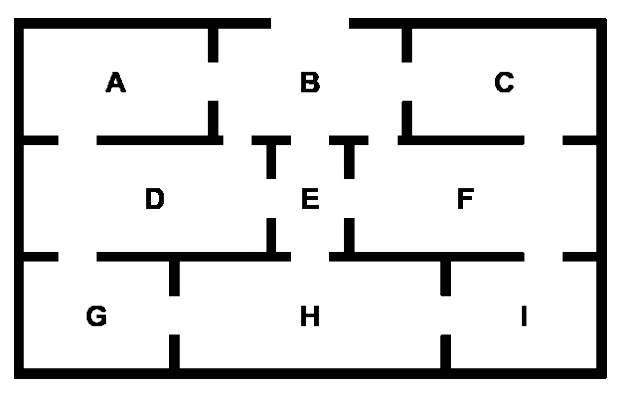
\includegraphics[width=0.5\linewidth]{content/Csurka_Molnar_Hanna-Kis_Aranka_Eniko-Gergely_Verona/betoro2.png}
	\end{center}
\end{problem}
\begin{solution}
	Ábrázoljuk a bankot egy gráffal.
	A gráf csúcsai a bank helyiségei, az élet pedig a helyiségek közti ajtók.
	Ahhoz, hogy a bank bejáratát is ábrázoljuk, a bankon kívüli teret is jelöljük egy csúccsal, ez legyen $O$ és a bejárati ajtó a $B$ és $O$ csúcsokat összekötő él lesz.
	Ekkor a gráf csúcsainak fokszámai: $A-2, B-6, C-2, D-4, E-4, F-4, G-2, H-3, I-2, O-1$.
	
	Mivel a betörő kintről érkezett és valamelyik helyiségbe jutott úgy, hogy minden ajtón pontosan egyszer ment át, olyan vonalat keresünk a gráfban ami az $O$ csúcsból indul és minden élen pontosan egyszer halad át, vagyis egy Euler-vonalat.
	A csúcsok közül $O$ és $H$ fokszáma páratlan, a többi páros, így a keresett Euler-vonal végpontja csak a $H$ lehet.
	Adjunk meg egy ilyen vonalat: $O\rightarrow B\rightarrow A\rightarrow D\rightarrow B\rightarrow C\rightarrow F\rightarrow B\rightarrow E\rightarrow D\rightarrow G\rightarrow H\rightarrow E\rightarrow F\rightarrow I\rightarrow H$, amint a mellékelt ábrán is látható.
	\begin{center}
		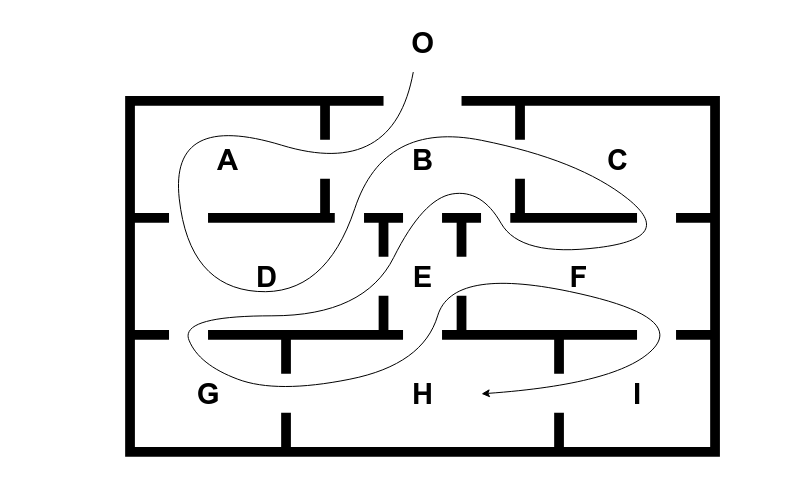
\includegraphics[width=0.5\linewidth]{content/Csurka_Molnar_Hanna-Kis_Aranka_Eniko-Gergely_Verona/betoro_megoldas.png}
	\end{center}
\end{solution}
\begin{problem}
	Lehetséges-e, hogy egy $N$ csúcsú gráfban a csúcsok fokszámai egymás után következő különböző pozitív egész számok?
\end{problem}
\begin{solution}
	Mivel nincs kikötve, hogy csak egyszerű gráfokkal dolgozhatunk, ezért a gráfban lehetnek párhuzamos- és hurokélek is.
	Tudjuk, hogy a fokszámok összege minden gráfban kétszerese az élek számának, ezért a fokszámok összegének páros számnak kell lennie.
	Páratlan darab páratlan fokszámú csúcsot tartalmazó gráfot nem rajzolhatunk.
	Páratlan csúcsszámú gráfok között meg tudunk adni olyan fokszámeloszlást, hogy a páratlan fokszámokból páros darab legyen:
	$N=4k+1$ esetén páros fokszámmal kezdve $2k+1$ darab páros és $2k$ darab páratlan fokszámú csúcs lesz;
	$N=4k+3$ esetén páratlan fokszámmal kezdve $2k+2$ darab páratlan és $2k+1$ darab páros fokszámú csúcs lesz.
	$N=4k$ esetén mindegy, hogy a fokszámok sozorata párossal, vagy páratlannal kezdődik, $2k$ darab páratlan fokszámú csúcs lesz.
	$N=4k+2$ esetén nem szerkeszthető meg a gráf, mivel $2k+1$ darab páratlan fokszámú csúcs kellene legyen benne.
	
	Páros fokszámú csúcs szerkeszthető $k$ darab hurokéllel, így $2k$ lesz a fokszáma.
	Páratlan fokszámú csúcsokat párba állítva szerkeszthetjük meg. Például a $2k-1$ és $2k+1$ fokszámú csúcsokat úgy állíthatjuk elő, hogy $2k-1$ párhuzamos élet húzunk közéjük és az egyik csúcsra még egy hurokélet szerkesztünk.
	Ezzel a szerkesztéssel tehát előállíthatunk olyan gráfot, amiben a csúcsok fokszámai egymásutáni különböző pozitív egész számok, amennyiben ezek a fokszámok között páros darab páratlan van.
\end{solution}
\begin{problem}
	Igazoljuk, hogy bármely gráfban az élek és a csúcsok számának hányadosa nagyobb vagy egyenlő, mint a minimális fokszámú csúcs fokszámának fele és kisebb vagy egyenlő, mint a maximális fokszámú csúcs fokszámának fele.
\end{problem}
\begin{solution}
	Legyen a gráf csúcsainak és éleinek száma rendre $N$ és $M$;
	a minimális és a maximális fokszámú csúcs fokszáma rendre $f$ és $F$.
	Ekkor a feladat bizonyítani a következő összefüggést:
	$$
	\frac{f}{2}\le\frac{M}{N}\le\frac{F}{2}.
	$$
	Végigszorozva az egyenlőtlenséget $2N$-el eltűnnek a törtek:
	$$
	N\cdot f \le 2\cdot M \le N\cdot F.
	$$
	Ez természetesen teljesül, mivel tudjuk, hogy $2\cdot M$ a gráf összes csúcsának fokszámainak összege.
	A fokszámok összege akkor lehet $N\cdot f$, ha minden csúcs fokszáma a minimális fokszámmal lenne egyenlő, de ennél kisebb nem lehet az összeg.
	Hasonló okból igaz a második egyenlőtlenség is.
	Egyenlőség csak egyszerre állhat fent, akkor ha a gráf minden csúcsának megegyezik a fokszáma.
\end{solution}
\begin{problem}
	Bizonyítsuk be, hogy egy $2N$ csúcsú egyszerű gráfban minden csúcs fokszáma legalább $N$, akkor a gráf összefüggő.
	Hány kört tartalmazhat maximum ez a gráf?
\end{problem}
\begin{solution}
	Tételezzük fel az állítás ellentétét.
	Tegyük fel, hogy van olyan gráf, amelynek $2N$ csúcsa van, és minden csúcs fokszáma legalább $N$, de a gráf legalább két komponensből áll.
	Mivel a gráfnak $2N$ csúcsa van, az egyik komponensbe biztosan legfeljebb $N$ csúcs jut.
	Mivel a gráf egyszerű, a komponensei is egyszerűek.
	
	Egy $N$ csúcsú egyszerű gráfban a maximális lehetséges fokszám egy csúcsban legfeljebb $N-1$, ami ellentmond annak a feltételnek, hogy minden csúcs fokszáma legalább $N$.
	Ezért az ellentmondás miatt az eredeti feltétel csak akkor teljesülhet, ha a gráf egy komponensből áll, vagyis összefüggő.
	
	Tehát egy $2N$ csúcsú egyszerű gráf, amelyben minden csúcs fokszáma legalább $N$, összefüggő.
\end{solution}
\begin{problem}
	Egy $N$ csúcsú egyszerű gráf minden csúcsának fokszáma $2$. Hány kört tartalmazhat maximálisan ez a gráf?
\end{problem}
\begin{solution}
	Ha minden csúcs fokszáma 2, akkor a gráf minden komponense kör.
	Az a célunk, hogy minél több kört tartalmazzon a gráf, ezért a lehető legtöbb rövid kört kell alkotni.
	A legrövidebb kör a háromcsúcsú kör.
	
	A kérdés tehát: hány háromcsúcsú (vagy egyéb rövid) körre bontható az $N$ csúcs?
	Példák:
	\begin{itemize}
		\item Ha \(n = 15\), akkor lehet öt darab három hosszú kör: \(5 \times 3 = 15\).
		\item Ha \(n = 16\), akkor lehet négy három- és egy négycsúcsú kör: \(4 \times 3 + 4 = 16\).
		\item Ha \(n = 17\), akkor lehet négy három- és egy ötcsúcsú kör: \(4 \times 3 + 5 = 17\).
	\end{itemize}
	
	Tehát az $N$ csúcsú egyszerű gráf maximális körszáma $\left\lfloor \frac{n}{3} \right\rfloor$.
\end{solution}


\section*{Nehezebb feladatok}

\begin{extraproblem}[Bartalis Dorottya]
Egy egyszerű, $N$ csúcsú gráfban minden csúcs fokszáma vagy $1$, vagy $3$. Tudjuk, hogy pontosan $k$ darab csúcsnak $1$ a fokszáma.


\begin{enumerate}
    \item Milyen feltételnek kell teljesülnie $N$ és $k$ között, hogy létezzen ilyen gráf?
    \item Mi a maximális lehetséges értéke $k$-nak, ha $N = 20$?
\end{enumerate}
\end{extraproblem}
\begin{solution}

\textbf{a)} Legyen $k$ az 1-fokú csúcsok száma. Ekkor a maradék $N - k$ darab csúcs fokszáma $3$.

A fokszámok összege:
\[
\sum \deg = 1 \cdot k + 3 \cdot (N - k) = k + 3N - 3k = 3N - 2k
\]
A fokszámösszegnek páros számnak kell lennie, mivel minden él két csúcshoz kapcsolódik:
\[
3N - 2k \equiv 0 \pmod{2}
\]
Mivel $2k$ páros, akkor $3N$-nek is párosnak kell lennie, azaz $N$-nek párosnak kell lennie.

Továbbá egy 3-fokú csúcs legfeljebb 3 darab 1-fokú csúcsot tud „kiszolgálni”, ezért:
\[
k \leq 3 \cdot (N - k)
\Rightarrow k \leq 3N - 3k
\Rightarrow 4k \leq 3N
\Rightarrow k \leq \frac{3N}{4}
\]

\textbf{Tehát:} akkor létezhet ilyen gráf, ha $N$ páros, és $k \leq \dfrac{3N}{4}$.

\vspace{1em}
\textbf{b)} Legyen $N = 20$.

Ekkor:
\[
k \leq \frac{3 \cdot 20}{4} = 15
\]
\[
\Rightarrow \boxed{k_{\max} = 15}
\]

Ez a határ éles: 15 darab 1-fokú csúcs kiszolgálásához pontosan 5 darab 3-fokú csúcs szükséges, mivel
\[
3 \cdot 5 = 15.
\]

A teljes gráfban tehát $k = 15$ darab 1-fokú és $N-k = 5$ darab 3-fokú csúcs van. A fokszámok összege:
\[
1 \cdot 15 + 3 \cdot 5 = 15 + 15 = 30,
\]
ami valóban páros, így egy ilyen gráf létezhet.
\end{solution}
\begin{extraproblem}[Csapó Hajnalka]
Egy baráti találkozó 9 résztvevője leírta, hogy hány emberrel fogott
kezet. A cédulákon ez állt: $1,2,3,4,5,4,3,2,1$ Lehetséges-e ez? 
\end{extraproblem}

\begin{solution}
Ha az emberek egy gráf csúcsai és a kézfogások az élek, akkor a kézfogások
száma a csúcsok fokszámai. A fokszámok összege: $1+2+3+4+5+4+3+2+1=25$.
De egy gráfban a fokszámok összege mindig páros, mert minden él két
csúcshoz tartozik, tehát nem lehetséges.
\end{solution}
\begin{extraproblem}[Csapó Hajnalka]
A cédulákon ezek a számok szerepelnek: $5,5,5,6,6,6,7,7,7$. Lehetséges-e
ez? 
\end{extraproblem}

\begin{solution}
Ebben az esetben a fokszámok összege páros, így megszerkesztjük a
gráfot.

\includegraphics[width=0.5\textwidth]{\string"content/Csurka_Molnar_Hanna-Kis_Aranka_Eniko-Gergely_Verona/9barat\string".JPG}
\end{solution}
\begin{extraproblem}[Gergely Verona]
Bizonyítsuk be, hogy nincs olyan tíztagú társaság, ahol az embereknek
rendre $9,9,9,8,8,8,7,6,4,4,$ ismerőse van! (Az ismeretségek kölcsönösek.)
\emph{(KöMaL, 1983) }
\end{extraproblem}

\begin{solution}
Tegyük fel, hogy mégis van a feladat feltételeit kielégítő társaság.
Legyenek az emberek egy gráf csúcspontjai, és az ismeretségek a gráfpontokat
összekötő élek.

Mivel három ember mindenkit ismer, ezért három csúcsot és a belőlük
kiinduló $9-9$ élt el is hagyhatunk a vizsgált gráfból. Elég belátni,
hogy a maradék gráf nem létezik, azaz nincs olyan 7 csúcsú gráf, ahol
a fokszámok rendre:

\[
5,\ 5,\ 5,\ 4,\ 3,\ 1,\ 1
\]

Legyen a két egyfokú csúcs $X$ és $Y$, az ötödfokú csúcsok pedig
$A$, $B$, $C$. Az $A$, $B$, $C$ csúcsok mindegyike egy híján
az összes többi ponttal össze van kötve, speciálisan $X$ és $Y$
közül is legalább eggyel.

Így $X$-ből és $Y$-ból összesen legalább 3 él indul, ami ellentmondás,
hiszen fokszámaik összege csupán $1+1=2$.

Így valóban nem létezik a feladatban leírt tíztagú társaság, ahogy
bizonyítanunk kellett. 
\end{solution}
\begin{extraproblem}[Kiss Andrea-Tímea]
Egy társaságban mindenki ismer legalább egy másik embert. Azt is
tudjuk, hogy ha két embernek azonos számú ismerőse van, akkor nincs
közös ismerősük. Igazoljuk, hogy van olyan ember, aki csak egy embert
ismer. 
\end{extraproblem}

\begin{solution}
Tekintsük a társaságot egy egyszerű, irányítatlan gráfként, ahol a
csúcsok az embereknek felelnek meg, és két csúcs között akkor van
él, ha az illető emberek ismerik egymást.

Legyen a társaságban $k+1$ ember, azaz a gráfban $k+1$ csúcs. Jelölje
$\deg(v)$ a $v$ csúcs fokát, vagyis hogy az adott személy hány másikat
ismer.

Tegyük fel indirekten, hogy mindenki legalább két embert ismer, vagyis
minden csúcs foka legalább $2$.

Válasszunk ki egy olyan $A$ személyt (csúcsot) , akinek a legtöbb
ismerőse van, azaz $\deg(A)=n$ maximális. Nyilván $n\leq k$, mivel
legfeljebb $k$ másik embert ismerhet.

Most nézzük meg $A$ ismerőseit. Ezek száma $n$, tehát $A$-hoz $n$
darab él tartozik. Az ismerősei közül azonban egyiknek sem lehet foka
$n$, hiszen:
\begin{itemize}
\item Ha $B$ olyan személy, akinek $\deg(B)=n$, akkor $\deg(A)=\deg(B)$. 
\item Mivel $A$ és $B$ ismerik egymást (hiszen $B$ $A$ egyik ismerőse),
ez ellentmond a feladat feltételének: két azonos fokszámú embernek
nem lehet közös ismerőse. 
\end{itemize}
Ezért $A$ minden ismerősének fokszáma legfeljebb $n-1$.

Továbbá, ha két embernek azonos fokszáma van, akkor nem lehet közös
ismerősük. Tehát $A$ legfeljebb egy olyan embert ismerhet, akinek
foka $i$, minden $i\leq n-1$ esetén. Ez azt jelenti, hogy $A$ legfeljebb
$n-1$ különböző fokszámú embert ismerhet.

Viszont $A$-nak pontosan $n$ ismerőse van, és azoknak a fokszáma
különböző kell legyen (különben lenne két azonos fokszámú ismerőse,
akiknek közös ismerőse $A$ lenne -- ez tilos). Ez ellentmondás:

\[
n\leq n-1\quad\text{– ez lehetetlen.}
\]

Ez az ellentmondás abból adódott, hogy feltételeztük: minden ember
legalább két embert ismer.

Tehát léteznie kell olyan embernek, aki csak egy másik embert ismer. 
\end{solution}
\begin{extraproblem}[Kovács Levente]
Adott egy város 6 pontja, amelyeket utakkal kell összekötni úgy,
hogy minden pontból el lehessen jutni bármely másikba, és az utak
teljes építési költsége minimális legyen. A költségek az alábbi szimmetrikus
táblázat szerint adottak:

\[
\begin{array}{c|cccccc}
 & A & B & C & D & E & F\\
\hline A & - & 4 & 2 & - & - & -\\
B & 4 & - & 1 & 5 & - & -\\
C & 2 & 1 & - & 8 & 10 & -\\
D & - & 5 & 8 & - & 2 & 6\\
E & - & - & 10 & 2 & - & 3\\
F & - & - & - & 6 & 3 & -
\end{array}
\]

Mely élekből áll a minimális feszítőfa (MST), és mi a teljes költsége? 
\end{extraproblem}

\vspace{1em}

\begin{solution}
A megoldáshoz a Kruskal-algoritmust alkalmazzuk, amely az éleket növekvő
sorrendbe rendezi súlyuk szerint:
\begin{itemize}
\item B--C: 1 
\item A--C: 2 
\item D--E: 2 
\item E--F: 3 
\item A--B: 4 
\item B--D: 5 
\item D--F: 6 
\item C--D: 8 
\item C--E: 10 
\end{itemize}
Az algoritmus lépései során az alábbi éleket választjuk ki (kört nem
alkotva):

\[
\text{Kiválasztott élek: B–C, A–C, D–E, E–F, A–B}
\]

Ez összeköti az összes csúcsot.

A teljes költség: 
\[
1+2+2+3+4=\boxed{12}
\]

Ez a minimális feszítőfa költsége. 
\end{solution}
\vspace{1em}

\begin{extraproblem}[Kovács Levente]
Adott egy irányítatlan gráf az alábbi élekkel: 
\[
\{A\text{–}B,A\text{–}C,B\text{–}C,B\text{–}D,C\text{–}D,D\text{–}E,E\text{–}F,F\text{–}C\}
\]
\begin{enumerate}
\item Van-e Euler-köre a gráfnak? 
\item Ha nincs, van-e Euler-út, és ha igen, adj meg egyet! 
\end{enumerate}
\end{extraproblem}

\vspace{1em}

\begin{enumerate}
\item Egy irányítatlan gráfban akkor és csak akkor van Euler-kör, ha összefüggő,
és minden csúcs foka páros.

Számoljuk meg a fokszámokat:
\begin{itemize}
\item $\deg(A)=2$ 
\begin{itemize}
\item $\deg(B)=3$ 
\item $\deg(C)=4$ 
\item $\deg(D)=3$ 
\item $\deg(E)=2$ 
\item $\deg(F)=2$ 
\end{itemize}
Mivel $B$ és $D$ foka páratlan, \textbf{nincs Euler-kör}.
\end{itemize}
\begin{enumerate}
\item Ha pontosan két csúcs foka páratlan, akkor van \textbf{Euler-út},
amely ezek között halad.

A gráf összefüggő, így Euler-út létezik.

Egy lehetséges Euler-út:

\[
A\rightarrow B\rightarrow C\rightarrow F\rightarrow E\rightarrow D\rightarrow C\rightarrow A
\]

Ez az út minden élt pontosan egyszer használ, de nem tér vissza a
kiindulóponthoz. 

\end{enumerate}
\end{enumerate}
\begin{extraproblem}[Lukács Andor]
Egy 9 tagú társaságban mindenki pontosan öt másik embernek átad 100
Ft-ot. Bizonyítsd be, hogy az ajándékozások után van két olyan ember,
akinek ugyanannyi forinttal változott a pénze! 
\end{extraproblem}

\begin{solution}
Az ajándékozást egy irányított gráf írja le, amelyben minden pont
kifoka 5. Ez alapján a gráfnak 45 éle van. Az élszám előáll úgy is,
mint a befokok összege. Ha két pont befoka ugyanaz, akkor a két megfelelő
ember pénze ugyanannyival változott. Így elég igazolni, hogy lesz
két olyan pont gráfunkban, amelyek befoka ugyanaz. Tegyük fel, hogy
ez nem igaz. Ekkor a kilenc befok különböző és a $\{0,1,2,\ldots,8\}$
halmazból kerül ki. Ez csak úgy lehet, hogy mindegyik lehetséges szám
pontosan egyszer fordul elő a befokok között. Ekkor viszont a befokok
összege $1+2+\cdots+8=36\neq45$, ami ellentmondás. Tehát létezik
két olyan pont, amelyek befoka azonos, így a két megfelelő személy
pénze is ugyanannyival változott. 
\end{solution}
\begin{extraproblem}[Lukács Andor]
Egy kocka éleit tetszőleges módon megszámozzuk az 1-től 12-ig terjedő
egész számokkal. Ezek után a kocka minden csúcsába felírjuk az ebbe
a csúcsba vezető élek számainak összegét. 
\begin{itemize}
\item[(a)] Bizonyítsd be, hogy a csúcsokhoz írt számok nem lehetnek mind egyenlők! 
\item[(b)] Vajon egyenlők lehetnek-e ezek az összegek, ha az egyik élre írt
számot 13-mal helyettesítjük? 
\item[(a)] Minden csúcshoz írjuk fel a háromtagú összeget. Az így kapott nyolc
összeget összeadva egy 24 tagú összeget kapunk, amelyben minden élhez
rendelt szám kétszer szerepel. Így az összeg értéke $2(1+2+\cdots+12)=12\cdot13$.
Ha mindegyik csúcsnál ugyanaz az összeg alakulna ki, akkor a közös
érték nyolcszorosát kellene kapnunk. $12\cdot13$ nem osztható nyolccal,
ami az állítást igazolja. 
\item[(b)] A növeléssel el kellene érnünk, hogy az előző rész megoldásában a
csúcsokhoz rendelt számok összege nyolccal osztható legyen. Ezt megtehetjük
úgy, hogy a 11-es számot cseréljük ki 13-ra. Az $1,2,\ldots,10,12,13$
számok hozzárendelése megfelelő élekhez egy ábrán könnyen megtalálható.
Tehát a válasz: igen, a csúcsokhoz rendelt értékek már egyenlők lehetnek. 
\end{itemize}
Tíz csapat körmérkőzést játszik. Mindegyik pár pontosan egyszer mérkőzik,
és a mérkőzések nem végződhetnek döntetlennel. Győzelemért 1 pont
jár, vereségért 0. Bizonyítsd be, hogy a csapatok pontszámainak négyzetösszege
nem lehet több 285-nél! 
\end{extraproblem}

\begin{solution}
Ha van két azonos $p$ pontszám (ekkor biztos, hogy $1\leq p\leq8$),
akkor a köztük lejátszott meccs eredményét megfordítva a módosított
bajnokságban ugyanazok a pontszámok alakulnak ki, kivéve a két $p$-s
pontszámot, amelyek $p-1$-gyé, illetve $p+1$-gyé válnak. Így a pontszámok
négyzetösszege nő. Tehát abban a bajnoki eredményben, amely maximalizálja
a pontszámok négyzetösszegét (ilyen biztos létezik, hiszen véges sok
lehetőség van a pontszámok kialakulására) minden pontszám különböző.
Ekkor viszont pontosan a $0,1,2,\ldots,9$ pontszámok alakulnak ki,
és így a maximális négyzetösszeg $1^{2}+2^{2}+\cdots+9^{2}=285$. 
\end{solution}
\begin{extraproblem}[Sógor Bence]
Legyen $k\geq2$. Bizonyítsd be, hogy ha egy gráfban minden csúcs
foka legalább $k$, akkor található benne legalább $k+1$ hosszú kör. 
\end{extraproblem}

\begin{solution}
Vegyük észre, hogy a gráf tartalmaz egy legalább $k$ hosszú utat.
Legyen $A_{1}$ a kiindulócsúcs. Ennek a fokszáma $k$, legyen $A_{2}$
egy szomszédja. Ekkor $A_{2}$-nek van legalább $k-1$ éle, amelyik
nem egy $A_{i}$, $i<2$ csúccsal köti össze. Hasonlóan, a sort folytatva
az $A_{l}$, $l<k+1$ csúcsnak van legalább $k-l+1$ éle ami nem egy
$A_{i}$, $i<l$ csúcsra mutat. Tehát az $A_{1}A_{2}\dots A_{k+1}$
egy $k$ hosszú út a gráfban.

Legyen $A_{1}A_{2}\dots A_{m}$ a leghosszabb út a gráfban. $A_{1}$-ből
minden él valamilyen $A_{i}$-re mutat, mert különben lehetne egy
hosszabb utat szerkeszteni, ezt a külső pontot $A_{1}$ elé téve.
Mivel $A_{1}$ fokszáma legalább $k$, ezért létezik $A_{l}$, $l\geq k+1$
úgy, hogy van él $A_{l}$ és $A_{1}$ között, de akkor az $A_{1}A_{2}\dots A_{l}A_{1}$
egy legalább $k+1$ hosszúságú kör. 
\end{solution}
\begin{extraproblem}[Száfta Antal]
Legyen $G$ egy egyszerű, összefüggő, nem irányított gráf $n$ csúccsal
és $n$ éllel. Tegyük fel, hogy: 
\begin{itemize}
\item $G$ nem tartalmaz 4-nél hosszabb kört, 
\item minden csúcs fokszáma legalább 2. 
\end{itemize}
\begin{enumerate}
\item[(a)] Igaz-e, hogy $G$ izomorfia szerint egyértelműen meghatározott? 
\item[(b)] Hány izomorfia szerint különböző gráf létezik ilyen feltételekkel,
ha $n=6$? 
\end{enumerate}
\end{extraproblem}

\begin{solution}
~

\textbf{1. Szerkezeti megfigyelés}\\
Egy $n$-csúcsú, összefüggő gráf $n$ éllel pontosan egy kört tartalmaz.

Mivel minden kör legfeljebb 3 hosszú, a gráf körének hossza pontosan
3, azaz háromszög.

\textbf{2. Fokszámfeltétel}\\
Minden csúcs fokszáma legalább 2. Ez kizárja azokat a bővítéseket,
amelyek csak egy éllel kapcsolódnak (levelek).

\textbf{3. Az (a) kérdés megválaszolása}\\
Nem. A fenti feltételek nem határozzák meg a gráfot egyértelműen izomorfia
szerint. Többféle módon is lehet három további csúcsot kapcsolni a
háromszöghöz, úgy hogy a feltételek teljesüljenek.

\textbf{4. Az (b) kérdés megválaszolása}\\
$n=6$ esetén pontosan egy háromszög van, és három további csúcs.

Az egyéb csúcsokat többféleképpen lehet csatlakoztatni a háromszöghöz
úgy, hogy: 
\begin{itemize}
\item a gráf összefüggő marad, 
\item ne keletkezzen újabb kör, 
\item minden csúcs fokszáma legalább 2. 
\end{itemize}
Részletes vizsgálattal két különböző, izomorfia szerint nem ekvivalens
gráf építhető fel.

\textbf{5. Válaszok:}
\begin{itemize}
\item[(a)] \textbf{Nem}, a gráf nem meghatározott egyértelműen izomorfia szerint. 
\item[(b)] $\boxed{2}$ különböző gráf létezik $n=6$ esetén. 
\end{itemize}
\end{solution}


\section{Síkgráfok, Euler-formula}\label{sec:sikgrafok}
\begin{description}
	{\large \item [{Szerző:}] Kis Aranka Enikő (Didaktikai mesteri -- Matematika, I. év) }
\end{description}
Elméleti összefoglaló: 
\begin{itemize}
	\item \textbf{Összefüggő gráf}: Egy gráf összefüggő, ha bármely két csúcsa
	között létezik út. 
	\item \textbf{Síkgráf}: Olyan gráf, amely lerajzolható a síkban úgy, hogy
	élei csak csúcsokban metszik egymást. 
	\item \textbf{Tartomány (régió)}: A síkgráf élei a síkot tartományokra (területekre)
	osztják. A külső régió is számít. 
	\item \textbf{Euler-formula síkgráfokra}: Ha egy síkgráf összefüggő és van
	benne: $n$ csúcs, $e$ él, $f$ tartomány, akkor: $n-e+f=2$
\end{itemize}

\section*{Házi feladatok}
\begin{problem}
	Igaz-e, hogy ha egy $n$ csúcsú gráfnak legfeljebb $3n-6$ éle van,
	akkor biztosan síkba rajzolható? (Ha igaznak találod, bizonyítsd;
	ha hamisnak találod, keress rá egy ellenpéldát.) 
\end{problem}

\begin{solution}
	Nem, például a $K_{3,3}$ gráfnak $n=6$ csúcsa van és $9=\left\lvert E\right\rvert \leq3\cdot6-6=12$,
	mégsem síkba rajzolható.
\end{solution}
\begin{problem}
	Síkba rajzolhatóak-e az alábbi (1.0.1 ábra) gráfok? Nemleges válasz
	esetén Kuratowski tételét használd az indokláshoz! 
	\begin{center}
		\includegraphics[width=0.8\linewidth]{\string"content/Csurka_Molnar_Hanna-Kis_Aranka_Eniko-Gergely_Verona/2.feladat\string".png}
	\end{center}
\end{problem}

\begin{solution}
	Az első és a harmadik gráfok síkba rajzolhatóak az ábra tanúsága szerint.
	(Persze az eredeti lerajzolásuk nem jó, de a síkba rajzolhatósághoz
	az kell, hogy le lehessen rajzolni élkeresztezés nélkül.) \textbf{Figyelem!}
	A harmadik ábra \emph{nem} soros bővítése a $K_{5}$-nek, mert a $K_{5}$
	két élét egyazon csúccsal osztottuk föl, ami nem megengedett soros
	bővítés esetén. A második gráf maga $K_{3,3}$ (az \{1; 2; 3\} és
	\{A; B; C\} csúcsosztályokkal), tehát nem síkba rajzolható. A negyedik
	gráfban az 1, 2, 3 és az A, B, C csúcsok közül bármely kettő között
	van út (a 2 és a C csúcsok között az $X$ nevű csúcson keresztül,
	a többi közt él van), tehát a gráf tartalmazza $K_{3,3}$ felosztását
	(más szavakkal élosztását, soros bővítését), így nem síkba rajzolható.
	A Petersen-gráf sem síkba rajzolható, mert tartalmazza a $K_{3,3}$
	felosztását. (Az ábrán a jobb láthatóság kedvéért kék, zöld, illetve
	piros színű élek jelzik az 1-es, a 2-es, illetve a 3-as csúcsokból
	az A, B, C-hez vezető utakat, és a felosztásban szereplő csúcsok is
	megfelelő színt kaptak, hogy jól látható legyen, hogy mindegyik csak
	egy felosztott élen szerepel.)
	
	Az ábra:
	\begin{center}
		\includegraphics[width=0.8\linewidth]{\string"content/Csurka_Molnar_Hanna-Kis_Aranka_Eniko-Gergely_Verona/2.feladat-megoldas\string".png}
	\end{center}
\end{solution}
\begin{problem}
	Igazoljuk, hogy bármely gráf vagy a komplementere összefüggő. 
\end{problem}

\begin{solution}
	Tegyük fel, hogy $G$ nem összefüggő. Legyen a gráf egy tetszőleges
	csúcsa $P$. A $P$-t tartalmazó komponens legyen $k$. $G$ komplementerében
	$P$-ből fut él a gráf összes $k$-n kívüli csúcsába. Ezek közül az
	egyik legyen $Q$ (k-n kívüli pont biztos van, mert $G$ nem összefüggő).
	
	$G$ komplementerében $Q$-ból fut él $k$ összes pontjába. Így $G$
	komplementerében tetszőleges két pont -- $P$ és $Q$-n keresztül
	-- legfeljebb három él hosszú úttal össze van kötve:
	\begin{itemize}
		\item Ha mindkét csúcs $k$-ban van, akkor mindkettő össze van kötve $Q$-val. 
		\item Ha mindkét csúcs $k$-n kívül van, akkor mindkettő össze van kötve
		$P$-vel. 
		\item Ha egyik $k$ egy pontja, a másik $k$-n kívüli csúcs, akkor az első
		össze van kötve $Q$-val, $QP$-vel, $P$ pedig a $k$-n kívüli ponttal. 
	\end{itemize}
\end{solution}
\begin{problem}
	Legyen $G$ egy egyszerű, összefüggő síkgráf, amelyben minden csúcs
	foka legalább 3, és minden lehatárolt (zárt) tartomány (azaz régió)
	legalább 5 oldalú. Mutasd meg, hogy az ilyen gráf csúcsainak száma
	legfeljebb kétharmada az élek számának, azaz: 
	\[
	n\leq\frac{2}{3}e,
	\]
	ahol $n$ a csúcsok száma és $e$ az élek száma. 
\end{problem}

\begin{solution}
	Legyen: 
	\begin{itemize}
		\item $n$: a gráf csúcsainak száma, 
		\item $e$: az élek száma, 
		\item $f$: a síkgráf régióinak (tartományainak) száma. 
	\end{itemize}
	Mivel $G$ síkgráf, ezért érvényes rá az Euler-formula: 
	\[
	n-e+f=2.
	\]
	
	\textbf{1. lépés:} Minden régió legalább 5 oldalú. \\
	Egy régió oldalainak száma megegyezik az azt határoló élek számával.
	Az összes régióra vonatkozóan tehát: 
	\[
	\text{Az összes régió összes oldala}\geq5f.
	\]
	Másrészt minden él pontosan két régió határához tartozik, így az összes
	oldal: 
	\[
	2e\geq5f\quad\Rightarrow\quad f\leq\frac{2}{5}e.
	\]
	
	\textbf{2. lépés:} Minden csúcs foka legalább 3. \\
	A fokszámok összege legalább $3n$, de ez egyenlő $2e$-vel (mivel
	minden él két csúcshoz kapcsolódik), tehát: 
	\[
	2e\geq3n\quad\Rightarrow\quad n\leq\frac{2}{3}e.
	\]
\end{solution}
\begin{problem}
	Ha $G$ $n$ csúcsú és $e$ éllel rendelkező síkba rajzolható gráf,
	és nem tartalmaz három hosszú kört, akkor 
	\[
	e\leq2n-4.
	\]
\end{problem}

\begin{solution}
	Ha $G$ egyszerű és nem tartalmaz három hosszú kört, akkor minden
	tartományt legalább 4 él határol, így: 
	\[
	4t\leq c_{1}+c_{2}+\dots+c_{t}\leq2e,
	\]
	amiből az előadásban látott számolással kapjuk, hogy 
	\[
	e\leq2n-4.
	\]
\end{solution}

\section*{Nehezebb feladatok}

\begin{extraproblem}[Bartalis Dorottya]
	Egy egyszerű, síkba rajzolható, \textbf{összefüggő} gráfban minden csúcs fokszáma legfeljebb 4, és a gráfnak $18$ éle van.
	
	\begin{enumerate}
		\item Legfeljebb hány csúcsa lehet a gráfnak?
		\item Lehetséges-e, hogy a gráf minden csúcsa pontosan 4-fokú?
	\end{enumerate}
\end{extraproblem}

\begin{solution}
	
	\textbf{1.} Legyen $n$ a csúcsok száma. Mivel egyszerű gráfról van szó, az élek száma $e = 18$.
	
	Az \textbf{Euler-formula} síkgráfokra:
	\[
	n - e + f = 2
	\]
	ahol $f$ a régiók (tartományok) száma.
	
	Továbbá a fokszámok összege:
	\[
	\sum \deg = 2e = 36
	\]
	Mivel minden csúcs fokszáma legfeljebb $4$, az összes fokszám legfeljebb $4n$:
	\[
	4n \geq 36 \Rightarrow n \geq 9
	\]
	
	Tehát a gráf \emph{legalább} 9 csúcsot tartalmaz. De a kérdés az volt: \emph{legfeljebb} hány csúcsa lehet?
	
	Mivel az élek száma rögzített ($e = 18$), a fokszámok összegének maximumát akkor kapjuk, ha \emph{minden csúcs foka a lehető legkisebb}, de legfeljebb 4. Tehát a legtöbb csúcs akkor lesz, ha minél több 1-fokú vagy 2-fokú csúcs van — de a gráf \textbf{összefüggő}, ezért csak 1-fokú csúcs nem lehet túl sok.
	
	Vegyük a legkedvezőbb (legnagyobb) $n$-t:
	\[
	2e = \sum \deg \leq 4n \Rightarrow 36 \leq 4n \Rightarrow n \geq 9
	\]
	
	De nincs felső korlát! Viszont a kérdés a \textbf{maximumra} vonatkozott. Ekkor úgy tekintünk rá, hogy minden csúcs foka legkisebb lehetőség: 1, 2, 3, stb.
	
	A legnagyobb lehetséges $n$ akkor van, ha a fokszámok a legkisebbek, de az összegük marad 36.
	
	Ekkor:
	\[
	\text{minimális fok: } 1 \Rightarrow \text{elméleti max } n = 36
	\]
	de 36 darab 1-fokú csúcsból nem építhető \textbf{összefüggő} gráf.
	
	Ha minden csúcs foka \textbf{2}, akkor:
	\[
	\sum \deg = 2n \Rightarrow 2n = 36 \Rightarrow n = 18
	\]
	Ez működőképes, például 18 csúcsból álló körrel (ez síkgráf).
	
	Tehát:
	\[
	\boxed{\text{A legtöbb csúcs: } \quad \boxed{18}}
	\]
	
	\medskip
	\textbf{2.} Lehetséges-e, hogy minden csúcs \textbf{pontosan 4-fokú}?
	
	Ha minden csúcs foka 4, akkor:
	\[
	\sum \deg = 4n = 2e = 36 \Rightarrow n = 9
	\]
	
	Most ellenőrizzük, létezik-e olyan síkba rajzolható, összefüggő egyszerű gráf, amelyben:
	- $n = 9$
	- $e = 18$
	- minden csúcs 4-fokú
	
	Vizsgáljuk meg az Euler-formulát:
	\[
	n - e + f = 2 \Rightarrow 9 - 18 + f = 2 \Rightarrow f = 11
	\]
	
	Nézzük a tartományokat: minden él legfeljebb 2 régiót határol, azaz a régiók oldalainak száma:
	\[
	\sum \text{oldalak} = 2e = 36
	\]
	11 régió 36 oldalból → az \emph{átlagos} tartomány 3.27 oldalú, azaz lehetséges.
	
	\textbf{Következtetés:}  
	\[
	\boxed{\text{Igen, létezhet olyan síkgráf, amelyben minden csúcs 4-fokú.}}
	\]
\end{solution}
\begin{extraproblem}[Csapó Hajnalka]
	Képzeljük el, hogy egy kocka élei \emph{gumiból} vannak!
	
	\textbf{a)} Belapítható-e a kocka a síkba úgy, hogy az élek illeszkedési
	viszonyai ne változzanak és ne metsszék egymást?
	
	\textbf{b)} Ugyanez a kérdés, ha két azonos méretű, \emph{lapszomszédos}
	kockánk van.
	
	\textbf{c)}Mi a helyzet akkor, ha egy kocka két szomszédos lapjához
	tettünk még egy-egy kockát?
	
	\textbf{d)}És akkor, ha egy közös él mentén van \emph{négy} kockánk?
\end{extraproblem}

\begin{solution}
	\textbf{a)} Igen.
	\begin{center}
		\includegraphics[width=0.5\textwidth]{\string"content/Csurka_Molnar_Hanna-Kis_Aranka_Eniko-Gergely_Verona/kockasikgraf\string".JPG}
	\end{center}
	
	\textbf{b)} Igen.
	\begin{center}
		\includegraphics[width=0.5\textwidth]{\string"content/Csurka_Molnar_Hanna-Kis_Aranka_Eniko-Gergely_Verona/2kocka\string".JPG}
	\end{center}
	
	\textbf{c)} Igen.
	\begin{center}
		\includegraphics[width=0.7\textwidth]{\string"content/Csurka_Molnar_Hanna-Kis_Aranka_Eniko-Gergely_Verona/3kocka\string".JPG}
	\end{center}
	
	\textbf{d)} Ebben az esetben találunk $K_{3,3}$-mal homeomorf részgráfot.
	\begin{center}
		\includegraphics[width=0.8\textwidth]{\string"content/Csurka_Molnar_Hanna-Kis_Aranka_Eniko-Gergely_Verona/4kockamegold\string".JPG}
	\end{center}
\end{solution}
\begin{extraproblem}[Csapó Hajnalka]
	Legyen egy gráf csúcsainak halmaza egy négyelemű halmaz kételemű
	részhalmazai. Azok között fut él, amelyeknek van közös eleme. Síkba
	rajzolható-e ez a gráf? 
\end{extraproblem}

\begin{solution}
	$A=\{1,2\},B=\{1,3\},C=\{1,4\},D=\{2,3\},E=\{2,4\},F=\{3,4\}$
	
	A gráf:
	
	\begin{center}
		\includegraphics[width=0.7\textwidth]{\string"content/Csurka_Molnar_Hanna-Kis_Aranka_Eniko-Gergely_Verona/reszhalmazok\string".JPG}
	\end{center}
	
	Ennek van $K_{3,3}$-mal homeomorf részgráfja.
\end{solution}
\begin{extraproblem}[Gergely Verona]
	Legyen $G$ olyan egyszerű gráf, amelyben minden csúcs foka legalább
	2. Mutassuk meg, hogy van $G$-nek olyan csúcsa, hogy minden belőle
	induló él benne van egy körben. \emph{(KöMaL, 2009) }
\end{extraproblem}

\begin{solution}
	Legyen a gráfban található leghosszabb út $L$, ennek egyik végpontja
	pedig $A$. Egy él már biztosan kiindul $A$-ból, ennek másik végpontját
	jelölje $B$. Mivel a gráfban minden csúcs fokszáma legalább $2$,
	azért $A$-ból legalább még egy további él kiindul. Egy ilyen él nem
	lehet hurokél, mert $G$ egyszerű gráf. Az él $A$-tól különböző végpontja
	$L$-ben kell hogy legyen, ellenkező esetben ugyanis lenne $L$-nél
	hosszabb út a gráfban. Legyen ez a végpont $C$. Az $L$-nek az $A$
	és $C$ csúcsot összekötő része (ami szintén út, és tartalmazza $B$-t)
	és az $AC$ él kört alkotnak. Ez bármely $A$-ból induló, $AB$-tól
	különböző élre elmondható. Az $AB$ él pedig az összes ilyen körben
	benne van. Így minden $A$-ból induló él benne lesz egy körben. Tehát
	az $A$ csúcs megfelelő. 
\end{solution}
\begin{extraproblem}[Kiss Andrea-Tímea]
	Egy $4n+2$ résztvevős bajnokságban eddig $2n$ számú fordulót rendeztek,
	azaz minden csapat $2n$ másik csapattal játszott. Igazoljuk, hogy
	van három olyan csapat, amelyek között még egyetlen mérkőzés sem volt. 
\end{extraproblem}

\begin{solution}
	Tegyük fel indirekten, hogy a $2n$ forduló után bármely három csapat
	között volt legalább egy mérkőzés.
	
	Válasszunk ki egy tetszőleges csapatot, és jelöljük $A$-val. Mivel
	$A$ eddig $2n$ másik csapattal játszott, a $4n+2$ csapatos mezőnyből
	$A$ még nem játszott:
	
	\[
	(4n+2)-1-2n=2n+1
	\]
	
	csapattal. Jelöljük ezt a $2n+1$ csapatból álló halmazt $S$-sel.
	Tehát $A$-nak a $S$ halmazban lévőkkel még nem volt mérkőzése.
	
	A feltevés szerint azonban bármely három csapat között volt legalább
	egy mérkőzés. Ez azt jelenti, hogy a $S$ halmaz bármely három csapata
	között történt már legalább egy mérkőzés.
	
	Vizsgáljuk meg ezt közelebbről:
	
	Az $S$ halmaz $2n+1$ csapatból áll, ami páratlan szám. A feltevés
	szerint $S$ bármely három csapata közül kettő már játszott egymással,
	tehát ezek a csapatok egymás között nagyon sok mérkőzést bonyolítottak
	le. Ugyanakkor egy bajnoki forduló során minden csapat csak egyszer
	játszik, vagyis minden fordulóban a csapatok párokba rendeződnek.
	
	Ez viszont lehetetlen, mert a $S$ halmazban \emph{páratlan} számú
	csapat van. Egyetlen forduló alatt páratlan számú csapat nem tud egymás
	között párokba rendeződve játszani: mindig maradna egy csapat mérkőzés
	nélkül.
	
	Tehát lehetetlen, hogy a $2n+1$ csapat minden lehetséges hármasából
	legalább egy mérkőzés már lejátszásra került, hiszen ehhez olyan számú
	fordulóra lenne szükség, amely lehetővé tenné, hogy páratlan sok csapat
	teljesen „összejátsszon egymással”, ami ellentmond a fordulók szervezési
	szabályainak.
	
	Ez ellentmondás. Tehát a feltevésünk hamis: \emph{létezik három olyan
		csapat, amelyek között még egyetlen mérkőzés sem volt}. 
\end{solution}
\begin{extraproblem}[Kovács Levente]
	Legyen $G$ egy egyszerű, összefüggő gráf 8 csúccsal, amelyben az
	alábbi élek szerepelnek: 
	\[
	\{A\text{–}B,A\text{–}C,B\text{–}C,B\text{–}D,C\text{–}E,D\text{–}E,D\text{–}F,E\text{–}G,F\text{–}G,G\text{–}H\}
	\]
	\begin{enumerate}
		\item Határozd meg a gráf kromatikus számát! 
		\item Adj meg egy érvényes színezést ennyi színnel! 
	\end{enumerate}
\end{extraproblem}

\begin{solution}
	A gráf kromatikus száma a minimális színek száma, amellyel a csúcsokat
	úgy színezhetjük, hogy szomszédos csúcsok különböző színűek legyenek.
	
	Mivel a gráf tartalmaz háromszöget (például $A\text{–}B\text{–}C\text{–}A$),
	legalább 3 szín szükséges.
	
	Egy lehetséges színezési sorrend: $A,B,C,D,E,F,G,H$
	
	Színezés: 
	\[
	\begin{aligned}A & =1\\
		B & =2\\
		C & =3\\
		D & =1\\
		E & =2\\
		F & =2\\
		G & =3\\
		H & =1
	\end{aligned}
	\]
	
	Tehát a kromatikus szám $\boxed{3}$, és egy példa színezés: 
	\[
	A=1,\;B=2,\;C=3,\;D=1,\;E=2,\;F=2,\;G=3,\;H=1
	\]
	
\end{solution}

\begin{extraproblem}[Kovács Levente]
	Vizsgáljuk meg, hogy a következő 6 csúcsú gráfnak van-e Hamilton-köre!
	A gráf élei: 
	\[
	\{A\text{–}B,A\text{–}C,B\text{–}C,B\text{–}D,C\text{–}E,D\text{–}E,D\text{–}F,E\text{–}F,F\text{–}A\}
	\]
	
	Van-e benne Hamilton-kör, és ha igen, adj meg egyet! 
\end{extraproblem}

\vspace{1em}

\begin{solution}
	Egy gráfban Hamilton-kör akkor van, ha létezik olyan kör, amely minden
	csúcsot pontosan egyszer érint, majd visszatér a kiindulóponthoz.
	
	Próbáljuk meg kézzel felépíteni:
	
	\[
	A\rightarrow B\rightarrow C\rightarrow E\rightarrow D\rightarrow F\rightarrow A
	\]
	
	Ellenőrzés: 
	\begin{itemize}
		\item Minden él létezik. 
		\item Minden csúcs egyszer szerepel. 
		\item A kör A-ból indul és oda tér vissza. 
	\end{itemize}
	\textbf{Következtetés:} A gráfban létezik Hamilton-kör: 
	\[
	\boxed{A\rightarrow B\rightarrow C\rightarrow E\rightarrow D\rightarrow F\rightarrow A}
	\]
\end{solution}
\begin{extraproblem}[Lukács Andor]
	Egy pingpongbajnokságon a tíz résztvevő közül mindenki egyszer játszott
	mindenkivel. Az egyes versenyzők győzelmeinek és vereségeinek száma
	legyen rendre $x_{1},x_{2},\ldots,x_{10}$, illetve $y_{1},y_{2},\ldots,y_{10}$.
	Bizonyítsd be, hogy 
	\[
	x_{1}^{2}+\cdots+x_{10}^{2}=y_{1}^{2}+\cdots+y_{10}^{2}.
	\]
\end{extraproblem}

\begin{solution}
	Nyilván $x_{i}+y_{i}=9$ (pingpongban nem lehetséges döntetlen). Ezt
	felhasználva a bizonyítandó állítás az $x_{1}+\cdots+x_{10}=45$ alakra
	hozható. Ez nyilvánvaló abból, hogy $x_{1}+\cdots+x_{10}$ az összes,
	$C_{10}^{2}$ mérkőzés számát adja. 
	\begin{itemize}
		\item[(a)] Egy $n$-szöget ($n\geq4$) egymást nem metsző átlókkal háromszögekre
		bontunk. Definiálunk egy gráfot, ennek csúcsai a felbontás háromszögei.
		Két háromszöget összekötünk, ha van közös oldaluk. Bizonyítsd be,
		hogy a kapott gráf fa! 
		\item[(b)] Bizonyítsd be, hogy a fenti felosztásban legalább két olyan háromszög
		is van, amelynek két oldala is az eredeti sokszög oldalai közül kerül
		ki! 
	\end{itemize}
	(a) A felbontást megadó átlókat sorban húzzuk be. Minden átló behúzása
	egy tartományt két részre oszt. Így a behúzott átlók száma eggyel
	kevesebb, mint a kialakuló tartományok száma. A definiált $G$ gráfra
	ez azt jelenti, hogy $|E(G)|=|V(G)|-1$.
	
	Minden felbontásnak feleltessük meg az így értelmezett gráfot. Egy
	háromszögnek megfelelő csúcs legyen a háromszög súlypontjában: két
	szomszédos csúcs összekötését reprezentáló görbe legyen egy töröttvonal,
	amely csak a közös oldal felőzópontjában törik meg. Tegyük fel, hogy
	a$G$-ben van egy $C$ kör. Ekkor $C$-nek egy síkgörbe felel meg,
	és ez teljesen a kiinduló sokszög belsejében halad. A $C$-nek megfelelő
	görbének is lesz belseje, és ebben kell lennie a felosztás egy csúcsának.
	Ez ellentmond annak, hogy a felosztás csúcsai csak a sokszög eredeti
	csúcsai közül kerülhetnek ki. Tehát $G$-ben nincs kör.
	
	Azt kaptuk, hogy a $G$ gráfban nincs kör, és éleinek száma eggyel
	kevesebb, mint a pontjainak száma, tehát következik, hogy $G$ fa.
	
	(b) $G$-nek legalább két pontja van, és így van benne két elsőfokú
	csúcs. Ezek a keresett háromszögeket reprezentálják. 
\end{solution}
\begin{extraproblem}[Péter Róbert]
	Legyen $G$ egy egyszerű, összefüggő gráf $n$ csúccsal ($n\geq5$),
	melyre teljesül: 
	\begin{itemize}
		\item $G$ háromszögmentes, azaz nem tartalmaz $K_{3}$ részgráfot, 
		\item Minden csúcs foka legalább $\left\lfloor \frac{n}{2}\right\rfloor $. 
	\end{itemize}
	\textbf{Bizonyítsd be:} $G$ páros, és határozd meg az élek maximális
	számát! 
\end{extraproblem}

\begin{solution}
	A feladat szerint $G$ háromszögmentes, és minden csúcs foka legalább
	$\left\lfloor \frac{n}{2}\right\rfloor $.
	
	A háromszögmentesség azt jelenti, hogy nincs olyan három csúcs, amelyek
	páronként össze vannak kötve.
	
	Tegyük fel indirekten, hogy $G$ nem páros. Ekkor $G$ tartalmaz
	legalább egy páratlan hosszúságú kört. A legkisebb lehetséges páratlan
	kör a $C_{5}$, azaz ötkör.
	
	Ugyanakkor, ha minden csúcs foka legalább $\left\lfloor \frac{n}{2}\right\rfloor $,
	akkor a gráfban nagyon sok él van. Így nehéz úgy kapcsolni sok csúcsot,
	hogy ne alakuljon ki háromszög.
	
	Vegyünk egy tetszőleges csúcsot $v$. Mivel $\deg(v)\geq\left\lfloor \frac{n}{2}\right\rfloor $,
	$v$-nek sok szomszédja van. Ha ezen szomszédok közül bármely kettő
	össze lenne kötve, akkor háromszög alakulna ki $v$-vel, ellentmondás.
	Ezért $v$ szomszédsága független halmaz.
	
	Ez azt jelenti, hogy a gráf két részre osztható, ahol minden él az
	egyik részcsúcsból a másik részcsúcsba megy. Ez a páros gráf definíciója.
	
	\bigskip{}
	
	\textbf{Következtetés:} $G$ páros.
	
	\bigskip{}
	
	\textbf{Maximális él-szám:}
	
	Turán tétele szerint a háromszögmentes gráf maximális élszáma: 
	\[
	\max|E(G)|=\left\lfloor \frac{n^{2}}{4}\right\rfloor ,
	\]
	amit a teljes kétosztályú gráf (pl. $K_{\lfloor n/2\rfloor,\lceil n/2\rceil}$)
	valósít meg.
	
	\bigskip{}
	
	\textbf{Válasz:} $G$ páros, és maximálisan 
	\[
	\left\lfloor \frac{n^{2}}{4}\right\rfloor 
	\]
	élt tartalmazhat. 
\end{solution}
\begin{extraproblem}[Sógor Bence]
	Legyen $P$ egy konvex poliéder. Jelölje $L_{k}$ a $k$ csúcsú lapok
	számát minden $k\geq3$ esetén. Bizonyítsd be, hogy $3L_{3}+2L_{4}+L_{5}\geq12.$ 
\end{extraproblem}

\begin{solution}
	A kijelentés igazolásához használjuk az Euler-formulát. Ha $Cs$ a
	csúcsok, $E$ az élek és $L$ a lapok száma, akkor $Cs-E+L=2$. A
	feladat jelöléseit használva tudjuk, hogy: 
	\[
	L=L_{3}+L_{4}+L_{5}+L_{6}+\cdots
	\]
	\[
	E=\frac{1}{2}(3L_{3}+4L_{4}+5L_{5}+6L_{6}+\cdots)
	\]
	\[
	Cs\leq\frac{1}{3}(3L_{3}+4L_{4}+5L_{5}+6L_{6}+\cdots).
	\]
	A csúcsok számára vonatkozó egyenlőtlenség onnan jön, hogy minden
	csúcsban legalább 3 él fut össze. Tehát 
	\[
	2=Cs-E+L\leq\frac{1}{3}\sum_{k\geq3}kL_{k}-\frac{1}{2}\sum_{k\geq3}kL_{k}+\sum_{k\geq3}L_{k}=\sum_{k\geq3}\frac{6-k}{6}L_{k}
	\]
	Beszorozva 6-tal kapju, hogy 
	\[
	12\leq3L_{3}+2L_{4}+L_{5}-L_{7}-2L_{8}-\cdots\leq3L_{3}+2L_{4}+L_{5}.
	\]
	Ezzel igazoltuk a kért egyenlőtlenséget. 
\end{solution}
\begin{extraproblem}[Sógor Bence]
	Egy konvex poliéder minden csúcsában 1 ötszög és 2 hatszög találkozik.
	Hány ötszögből és hány hatszögből áll a poliéder? 
\end{extraproblem}

\begin{solution}
	Írjuk fel az Euler-formulát az előző feladat jelöléseit használva
	\[
	Cs=5\cdot L_{5}=3L_{6}
	\]
	\[
	E=\frac{1}{2}(5L_{5}+6L_{6})
	\]
	\[
	L=L_{5}+L_{6}.
	\]
	Ekkor 
	\[
	Cs-E+L=2\iff5L_{5}-\frac{1}{2}(5L_{5}+6L_{6})+L_{5}+L_{6}=2\iff7L_{5}-4L_{6}=4.
	\]
	Mivel $5L_{5}=3L_{6},$ ezért az alábbi módon alakíthatjuk az előző
	egyenletet: 
	\[
	7L_{5}-4L_{6}=4\iff21L_{5}-12L_{6}=12\iff21L_{5}-20L_{5}=12\iff L_{5}=12.
	\]
	Tehát $L_{5}=12$ és $L_{6}=20$. 
\end{solution}
\begin{extraproblem}[Száfta Antal]
	Legyen $G$ egy egyszerű, síkba rajzolható (planáris), összefüggő
	gráf, amely nem tartalmaz háromnál kisebb köröket, és minden csúcsa
	legalább fokszám 3. Tudjuk, hogy $G$-nek 12 csúcsa van.
	\begin{enumerate}
		\item[(a)] Legfeljebb hány éle lehet $G$-nek? 
		\item[(b)] Létezhet-e olyan síkba rajzolható gráf, amely pontosan ennyi élt
		tartalmaz, és nem tartalmaz háromszöget? 
	\end{enumerate}
\end{extraproblem}

\begin{solution}
	\textbf{1. Euler-formula alkalmazása}\\
	Síkba rajzolható összefüggő gráfra igaz:
	\[
	v-e+f=2
	\]
	Tegyük fel, hogy a gráf nem tartalmaz háromszöget. Ekkor minden régiót
	határoló kör legalább 4 hosszú.
	Ekkor az élek és régiók kapcsolata alapján:
	\[
	2e\geq4f\Rightarrow f\leq\frac{e}{2}
	\]
	Ezt visszahelyettesítve az Euler-formulába:
	\[
	v-e+f=2\Rightarrow v-e+\frac{e}{2}\geq2\Rightarrow v-\frac{e}{2}\geq2\Rightarrow e\leq2v-4
	\]
	
	\textbf{2. Konkrét számolás}\\
	Adott: $v=12$. Ekkor:
	\[
	e\leq2\cdot12-4=24-4=\boxed{20}
	\]
	
	\textbf{3. Létezik-e ilyen gráf?}\\
	Igen. Léteznek olyan síkba rajzolható gráfok, amelyek: 
	\begin{itemize}
		\item 12 csúcsból állnak, 
		\item minden körük legalább 4 hosszú, 
		\item és pontosan 20 élük van. 
	\end{itemize}
	Például rácsszerkezetre épülő síkgráf, négyszög-régiókkal.
	
	\textbf{Válaszok:}
	\begin{itemize}
		\item[(a)] A maximális él-szám: $\boxed{20}$ 
		\item[(b)] \textbf{Igen}, létezik ilyen gráf. 
	\end{itemize}
\end{solution}
\begin{extraproblem}[Szélyes Klaudia]
	Adott egy gráf $G$, melynek:
	\begin{itemize}
		\item $n=8$ csúcsa van, 
		\item $e=15$ éle van, 
		\item az élhalmaz a következő: 
		\[
		E=\{(1,2),(1,3),(1,4),(2,3),(2,5),(3,6),(4,5),(4,6),(5,6),(5,7),(6,8),(7,8),(3,7),(2,8),(1,7)\}
		\]
	\end{itemize}
	\noindent\textbf{Kérdések:} 
	\begin{enumerate}
		\item Rajzolható-e síkba ez a gráf? 
		\item Ha \emph{nem}, azonosíts benne egy \textbf{Kuratowski-algráfot} (például
		$K_{5}$ vagy $K_{3,3}$). 
		\item Ha \emph{igen}, vázold fel a síkbarajzolását élmetszés nélkül. 
	\end{enumerate}
\end{extraproblem}
\begin{solution}
	A síkbarajzolhatóság eldöntéséhez használhatjuk az \textbf{Euler-formulát}:
	\[
	n-e+f=2\quad\text{(összefüggő síkgráfra)}
	\]
	Az adott gráfban:
	\[
	n=8,\quad e=15
	\]
	Ha $G$ \emph{síkgráf lenne}, akkor a tartományok száma $f$:
	\[
	f=2-n+e=2-8+15=9
	\]
	Ez még nem ellentmondás, de vizsgáljuk meg a síkgráfokra vonatkozó
	ismert felső korlátot:
	\[
	e\leq3n-6=3\cdot8-6=18
	\]
	Ez szintén teljesül, tehát az él- és csúcsszám alapján \textbf{lehetséges
		lenne síkba rajzolni}. Azonban keressünk benne \textbf{nem síkbarajzolható
		részgráfot}.
	
	Vegyük az alábbi csúcshalmazokat: $\{1,2,3,5,7,8\}$. Ezen belül vizsgáljuk az éleket: 
	\[
	(1,2),(1,3),(2,3),(2,5),(5,7),(7,8),(2,8),(1,7),(3,7)
	\]
	Ez egy $K_{3,3}$ típusú elrendezést eredményezhet, ha felosztható
	két háromelemű csoportra úgy, hogy minden él a két csoport közül köt
	össze csúcsokat. Például:
	\[
	A=\{1,2,3\},\quad B=\{5,7,8\}
	\]
	És a köztük lévő élek:
	\[
	(2,5),(2,8),(1,7),(3,7),(1,5),(3,8)\quad\text{(teljes páros kapcsolatok megközelítése)}
	\]
	Egy ilyen részgráf már elegendő ahhoz, hogy következtessünk: a gráf
	tartalmaz \textbf{Kuratowski-algráfot}, azaz \textbf{nem síkba rajzolható}.
\end{solution}



\section{Térképek és gráfok színezése}\label{sec:terkepek}
\begin{description}
	{\large \item [{Szerző:}] Gergely Verona (Didaktikai mesteri -- Matematika, II. év) }
\end{description}

\begin{definition}{def:sikgraf}
	Legyen $G$ egy gráf és $k\geq1$ egész szám.
	A $G$ gráf $k$ színnel színezhető, ha a $G$ minden csúcsa kiszínezhető
	$k$ adott (tetszőleges) színnel úgy, hogy $G$ bármely két szomszédos
	csúcsának a színe különböző. A $G$ kromatikus száma $k$, ha a $G$
	gráf $k$ színnel színezhető, de $(k-1)$-gyel már nem. $G$ kromatikus
	számának a jele:$\chi(G)$.
\end{definition}
\begin{definition}{def:bipartite}
	A $G$ gráfot páros gráfnak nevezzük, ha a $V(G)$
	csúcshalmaza felbontható az $A$ és $B$ diszjunkt halmazok egyesítésére
	úgy, hogy a $G$ minden éle egy $A$-beli csúcsot köt össze egy $B$-belivel.
\end{definition}
\begin{theorem}{thm:bipartite-color}
	Egy gráf pontosan akkor páros gráf (kiszínezhető két színnel), ha
	nem tartalmaz páratlan hosszúságú kört. 
\end{theorem}
\begin{proof}
	A feltétel valóban szükséges. Az elégségesség igazolásához tegyük
	fel, hogy gráfunkban nincs páratlan hosszúságú kör. 
	\begin{center}
		\includegraphics[scale=0.37]{\string"content/Csurka_Molnar_Hanna-Kis_Aranka_Eniko-Gergely_Verona/paros_graf_biz\string".png} 
		\par\end{center}
	Algoritmus: 
	\begin{enumerate}
		\item Jelöljük ki a gráf egy tetszőleges $a$ pontját, és színezzük feketére. 
		\item Színezzük $a$ minden szomszédját fehérre.($a$ szomszédai nem lehetnek
		összekötve) 
		\item Ezután színezzük ez utóbbi pontok minden - eddig ki nem színezett
		- szomszédját feketére. 
	\end{enumerate}
	Be kell bizonyítanunk, hogy nincs olyan él, amely két fekete pontot
	köt össze.
	
	Az $a$ pont és az újonnan berajzolt fekete pontok között nem halad
	él, mivel az utóbbiak nem szomszédjai $a$-nak. Az újonnan feketére
	festett pontok között sem haladhat él, így ugyanis vagy 3, vagy 5
	hosszúságú kör jönne létre.
	
	Ha a gráf összefüggő, akkor az eljárást folytatva valamennyi pontot
	kiszínezhetjük két színnel. Könnyen belátható, hogy két azonos színű
	pont között nem haladhat él.
	
	\smallskip{}
	
	Indirekt bizonyítunk: tegyük fel tehát, hogy az $u$ és $v$ szomszédos
	pontok (mondjuk) egyaránt feketék. Az u pont szomszédjai között van
	olyan $u$, amelyet az $u$-t megelőző körben színeztünk ki (így nyilván
	fehér), $u_{1}$-nek van olyan $u_{2}$ szomszédja, amelyet ezt megelőzőleg
	(és így feketére) színeztünk ki. Az eljárást folytatva olyan $P$
	utat kapunk, amely $u$-ból az $a$ kezdőpontba vezet. Hasonlóan kaphatunk
	egy a $v$-ből az $a$ kezdőpontba vezető $Q$ utat. Ha most $u$-ből
	elindulunk $Q$-n, addig megyünk, amíg először el nem érjük $P$-t,
	ezután $P$-t követjük $u$-ig, végül az $uv$ élen haladunk, akkor
	egy kört kapunk. Mivel $u$-ból indulva a kör mentén haladva a pontok
	színe váltakozik, $u$ és $v$ viszont egyaránt fekete, a kör páratlan
	számú élből kell hogy álljon - ez pedig ellentmond a feltételünknek.
	
	Ha a gráf összefüggő, akkor meg is vagyunk, hiszen minden pontját
	kiszíneztük. Ha nem, akkor színezzük külön-külön az összefüggő komponenseket
	ugyanezzel a módszerrel. 
\end{proof}
\begin{definition}{def:klikk}
	A $G$ gráf klikkszáma $k$, ha $G$-ben található
	$k$ darab csúcs úgy, hogy ezek közül bármely kettő szomszédos, de
	$k+1$ ilyen csúcs már nem található. G klikkszámának a jele: $\omega(G)$.
\end{definition}
\begin{theorem}{thm:hurokelmentes}
	Minden G (hurokélmentes) gráfra $\chi(G)\leq\Delta(G)+1$, ahol $\Delta(G)$
	a $G$-beli maximális fokszámot jelöli. 
\end{theorem}

\textbf{A kromatikus szám ($\chi(G)$) néhány tulajdonsága:} 
\begin{itemize}
	\item $\chi(G)=1\Leftrightarrow$ a gráf csúcsai páronként szomszédosak
	- azaz $G$ izolált pontokból áll. 
	\item $\chi(G)=2$, ha $G$ páros gráf. 
	\item $\chi(G)\geq3$, ha $G$ tartalmaz páratlan kört. 
	\item $\chi(G)\geq\omega(G)$, ahol $\omega(G)$ a $G$ gráf klikkszáma. 
	\item Ha $\chi(G)=\omega(G)$, akkor a $G$ gráfot perfektnek nevezzük. 
\end{itemize}
\begin{theorem}{thm:negyszin}
	Minden síkba rajzolható gráf kiszínezhető négy színnel. 
\end{theorem}


\section*{Házi feladatok}
\begin{problem}
	Adott a következő gráf. Határozzuk meg:
	
	a) Páros-e a gráf? Válaszodat indokold!
	
	b) Mennyi a gráf kromatikus száma? 
	\begin{center}
		\includegraphics[scale=0.6]{\string"content/Csurka_Molnar_Hanna-Kis_Aranka_Eniko-Gergely_Verona/Petersen1_tiny.svg\string".png} 
		\par\end{center}
\end{problem}

\begin{solution}
	a) Az adott gráf nem páros, mivel tartalmaz $5$ hosszúságú
	kört.
	
	b) Mivel a gráf nem páros, vagyis nem színezhető ki $2$ színnel,
	ezért $\chi(G)\geq3$. Egy lehetséges színezés $3$ színnel:
	\begin{center}
		\includegraphics[scale=0.3]{\string"content/Csurka_Molnar_Hanna-Kis_Aranka_Eniko-Gergely_Verona/Petersen_graph_3-coloring.svg\string".png} 
		\par\end{center}
	Mivel a gráf nem színezhető ki $2$ színnel, de $3$ színnel igen,
	ezért a kromatikus száma $\chi(G)=3$. 
\end{solution}
\begin{problem}
	Határozzuk meg az alábbi $G$ gráfok $\omega(G)$ klikkszámát
	és $\chi(G)$ kromatikus számát! 
	\begin{center}
		\includegraphics[scale=0.5]{\string"content/Csurka_Molnar_Hanna-Kis_Aranka_Eniko-Gergely_Verona/feladat2\string".png} 
		\par\end{center}
\end{problem}

\begin{solution}
	A bal oldali gráfban könnyű találni egy $4$-es klikket,
	például $a$, $b$, $f$ és $e$. Ebből következik, hogy $\chi(G)\geq\omega(G)=4$,
	vagyis három színnel nem színezhető ki. Ezért a sejtésünk az, hogy
	négy színnel kiszínezhető, egy példa erre:
	\begin{center}
		\includegraphics[scale=0.5]{\string"content/Csurka_Molnar_Hanna-Kis_Aranka_Eniko-Gergely_Verona/feladat2-1-m\string".png} 
		\par\end{center}
	Tehát mivel a gráf nem színezhető ki 3 színnel, de 4-gyel igen, ezért
	$\chi(G)=4$.
	
	A jobb oldali gráfban pedig látható, hogy tartalmaz egy páratlan hosszúságú
	kört ($b$--$c$--$g$--$f$--$e$--$b$), vagyis $\chi(G)>2$.
	Próbáljuk meg kiszínezni 3 színnel.
	\begin{center}
		\includegraphics[scale=0.5]{\string"content/Csurka_Molnar_Hanna-Kis_Aranka_Eniko-Gergely_Verona/feladat2-2-m\string".png} 
		\par\end{center}
	Másrészt ránézésre is jól látszik, hogy ebben a gráfban nincs háromszög
	(vagyis három csúcsú klikk). Két csúcsú klikk viszont nyilván van:
	bármelyik él két végpontja ilyen klikket alkot. Ezért $\omega(G)=2$. 
\end{solution}
\begin{problem}
	Igazoljuk, hogy a síkban véges sok egyenes által alkotott
	térkép két színnel színezhető. 
\end{problem}

\begin{solution}
	A feladatot indukcióval oldjuk meg.
	
	\textbf{Állítás (P(n)):} A síkban elhelyezett $n$ darab egyenes által
	meghatározott tartományok két színnel kiszínezhetők úgy, hogy szomszédos
	tartományok különböző színűek legyenek.
	
	\textbf{Alapeset (n = 0):} Ha nincs egyenes a síkon, akkor a sík egyetlen
	tartományból áll, amit bármely színnel kiszínezhetünk. Az állítás
	tehát teljesül.
	
	\textbf{Indukciós feltevés:} Tegyük fel, hogy az állítás igaz $n=k$
	esetén, azaz $k$ darab egyenes által alkotott térkép két színnel
	helyesen színezhető.
	
	\textbf{Indukciós lépés:} Vizsgáljuk meg, hogy az állítás igaz marad-e,
	ha a térképhez hozzáadunk egy új, $k+1$-edik egyenest.
	
	Az indukciós feltevés szerint a $k$ darab egyenes által meghatározott
	régiókat két színnel kiszíneztük úgy, hogy szomszédos régiók különböző
	színűek.
	\begin{center}
		\includegraphics[width=0.5\textwidth]{\string"content/Csurka_Molnar_Hanna-Kis_Aranka_Eniko-Gergely_Verona/indukcio\string".png} 
		\par\end{center}
	Most vegyük az új egyenest (lilla egyenes az ábrán), amely felosztja
	a síkot két félsíkra, és a meglévő régiók egy részét kettévágja. Az
	új egyenes egyik oldalán megtartjuk a meglévő színezést, a másik oldalon
	viszont \textit{felcseréljük} a színeket (a fehéret kékre, a kéket
	fehérre változtatjuk).
	
	Ez a színcsere biztosítja, hogy az új egyenes által szétválasztott
	régiók különböző színt kapjanak. Azok a régiók pedig, amelyeket az
	új egyenes nem érint, továbbra is jól vannak színezve az indukciós
	feltevés miatt.
	\begin{center}
		\includegraphics[width=0.5\textwidth]{\string"content/Csurka_Molnar_Hanna-Kis_Aranka_Eniko-Gergely_Verona/indukcio+1\string".png} 
	\end{center}
	\medskip{}
	
	\textbf{Következtetés:} Az új egyenes is minden szomszédos régióra
	különböző színt rendel, tehát az állítás $k+1$ esetén is igaz. Ekkor
	a matematikai indukció alapján az állítás minden $n\in\mathbb{N}$
	esetén teljesül. 
\end{solution}
\begin{problem}
	Egy egyetemen a következő tantárgy-pároknak vannak közös
	hallgatóik: 1 és 2, 1 és 3, 1 és 4, 1 és 7, 2 és 3, 2 és 4, 2 és 5,
	2 és 7, 3 és 4, 3 és 6, 3 és 7, 4 és 5, 4 és 6, 5 és 6, 5 és 7, 6
	és 7.
	
	Hogyan lehet úgy beosztani a záróvizsgákat az egyetemen, hogy egyetlen
	hallgatónak se legyen két vizsgája egyszerre? 
\end{problem}

\begin{solution}
	A feladatot gráfokra írjuk át: a különböző tantárgyak a
	gráf csúcsait fogják jelölni, az élek pedig azt jelzik, ha két tantárgy
	között van közös hallgató. Így átírva a feladatot, a következő gráfot
	kapjuk:
	\begin{center}
		\includegraphics[width=0.5\textwidth]{\string"content/Csurka_Molnar_Hanna-Kis_Aranka_Eniko-Gergely_Verona/feladat3\string".png} 
		\par\end{center}
	Ahhoz, hogy jól tudjuk beosztani a záróvizsgákat, azt kell megvizsgálnunk,
	hogy az adott gráf hány színnel színezhető ki. Látható, hogy a gráf
	tartalmaz egy $4$ méretű klikket, például az $1,2,3,7$, vagyis $\chi(G)\geq\omega(G)=4$.
	Ez azt jelenti, hogy a gráf nem színezhető ki három színnel.
	
	Ha találunk egy megfelelő színezést négy szín felhasználásával, akkor
	meg is van az optimális beosztás --- és valóban, találunk ilyet:
	\begin{center}
		\includegraphics[scale=0.55]{\string"content/Csurka_Molnar_Hanna-Kis_Aranka_Eniko-Gergely_Verona/feladat3sz\string".png} 
		\par\end{center}
	Tehát $\chi(G)=4$. Ezek alapján egy optimális záróvizsgabeosztás
	például a következő lehet:
	\begin{center}
		\begin{tabular}{|c|c|}
			\hline 
			\textbf{Időbeosztás}  & \textbf{Tantárgyak} \tabularnewline
			\hline 
			I.  & 2, 6 \tabularnewline
			II.  & 1 \tabularnewline
			III.  & 3, 5 \tabularnewline
			IV.  & 4, 7 \tabularnewline
			\hline 
		\end{tabular}
		\par\end{center}
\end{solution}
\begin{problem}
	(Vasárnapi Újság rejtvényrovata -- 1912). Melyik az a négy
	magyarországi megye (1912-es térképen), melyek bármelyikéből a többi
	három megye bármelyikébe közvetlenül el lehet jutni, azaz a nélkül,
	hogy egy harmadik megyén kelljen áthaladni? Található-e Magyarországon
	öt megye ugyanezzel a tulajdonsággal? 
	\begin{center}
		\includegraphics[scale=0.5]{\string"content/Csurka_Molnar_Hanna-Kis_Aranka_Eniko-Gergely_Verona/Kingdom_of_Hungary_counties.svg\string".png} 
		\par\end{center}
\end{problem}

\begin{solution}
	Írjuk át a feladatot gráfokra: Minden megye egy csúcspontnak
	felel meg. Élt akkor húzunk két csúcs közé, ha az adott megyék szomszédosak
	a térképen.
	
	Így az első kérdés a következőképpen értelmezhető: keressünk egy 4
	csúcsú klikket (teljes részgráfot) a megyék szomszédsági gráfjában.
	
	Így a következő gráfot kapjuk:
	\begin{center}
		\begin{minipage}[c]{0.45\textwidth}%
			\centering \includegraphics[width=1\linewidth]{\string"content/Csurka_Molnar_Hanna-Kis_Aranka_Eniko-Gergely_Verona/grafok\string".png} %
		\end{minipage}\hfill{}%
		\begin{minipage}[c]{0.45\textwidth}%
			\centering \includegraphics[width=1\linewidth]{\string"content/Csurka_Molnar_Hanna-Kis_Aranka_Eniko-Gergely_Verona/tgraf\string".png} %
		\end{minipage}
		\par\end{center}
	Jól látható, hogy pontosan \textbf{egy} olyan részgráf van, amely
	$4$ csúcsú klikket alkot: \textbf{Bereg, Ugocsa, Máramaros és Szatmár}.
	\begin{center}
		\begin{minipage}[c]{0.45\textwidth}%
			\centering \includegraphics[width=1\linewidth]{\string"content/Csurka_Molnar_Hanna-Kis_Aranka_Eniko-Gergely_Verona/tgrafklikk\string".png} %
		\end{minipage}\hfill{}%
		\begin{minipage}[c]{0.45\textwidth}%
			\centering \includegraphics[width=1\linewidth]{\string"content/Csurka_Molnar_Hanna-Kis_Aranka_Eniko-Gergely_Verona/terkepklikk\string".png} %
		\end{minipage}
		\par\end{center}
	\vspace{0.5cm}
	
	A feladat második része arra kérdez rá, hogy létezik-e öt olyan megye,
	amelyek mind páronként szomszédosak. Ez gráfelméletileg egy $K_{5}$
	klikket jelentene. Azonban ez \textbf{lehetetlen}, mivel az \textbf{ötcsúcsú
		teljes gráf nem síkba rajzolható élmetszés nélkül}, azaz \textbf{nem
		síkgráf}. Mivel a megyék térképe természetes módon síkgráf, ilyen
	klikk nem fordulhat elő.
	
	\bigskip{}
	
	\textbf{Extra:} A térkép, vagyis a gráf \textbf{4 színnel színezhető}
	úgy, hogy bármely megye szomszédai különböző színűek legyenek.
	\begin{center}
		\begin{minipage}[c]{0.45\textwidth}%
			\centering \includegraphics[width=1\linewidth]{\string"content/Csurka_Molnar_Hanna-Kis_Aranka_Eniko-Gergely_Verona/terkepsz2g\string".png} %
		\end{minipage}\hfill{}%
		\begin{minipage}[c]{0.45\textwidth}%
			\centering \includegraphics[width=1\linewidth]{\string"content/Csurka_Molnar_Hanna-Kis_Aranka_Eniko-Gergely_Verona/terkepsz2\string".png} %
		\end{minipage}
		\par\end{center}
\end{solution}

\section*{Nehezebb feladatok}
\begin{extraproblem}[Kiss Andrea-Tímea]
	Legyen $G$ egy gráf, amelynek csúcsai az $1$ és $1000$ közé eső
	természetes számok. Két különböző csúcsot akkor kötünk össze éllel,
	ha a különbségük legfeljebb $9$. Határozzuk meg $G$ kromatikus számát,
	$\chi(G)$-t. 
\end{extraproblem}

\begin{solution}
	Figyeljük meg, hogy minden $v\in\{1,2,\dots,1000\}$ csúcs össze van
	kötve azokkal a csúcsokkal, amelyek legfeljebb $9$-cel kisebbek vagy
	nagyobbak nála (feltéve, hogy ezek az értékek 1 és 1000 között vannak).
	
	Ezért minden csúcs fokszáma legfeljebb $18$ (kivéve a szélső értékeknél,
	ahol kevesebb szomszéd lehet).
	
	Konstruktív színezés 10 színnel: színezzük az összes olyan csúcsot,
	amely $10$-zel osztva ugyanazt a maradékot adja, ugyanazzal a színnel.
	Formálisan, minden $v$ csúcsot színezzünk:
	
	\[
	\text{színe}(v)=v\mod 10\quad\text{(és a 0 maradékot tekintsük 10-es színnek)}.
	\]
	
	Így például: 
	\begin{itemize}
		\item az $1$, $11$, $21$, $31$, $\dots$ számokat 1-es színnel, 
		\item a $2$, $12$, $22$, $\dots$ számokat 2-es színnel, stb., 
		\item a $10$, $20$, $30$, $\dots$ számokat 10-es színnel színezzük. 
	\end{itemize}
	Megfigyelés: két azonos színű csúcs különbsége legalább $10$, tehát
	ők nem lehetnek szomszédosak a gráfban (hiszen csak a legfeljebb $9$
	különbség esetén húzunk élt). Ez tehát \emph{helyes színezés} 10 színnel.
	
	Ez alapján: 
	\[
	\chi(G)\leq10.
	\]
	
	Most mutassuk meg, hogy kevesebb, mint 10 szín nem elég.
	
	Vegyük például a következő 10 csúcsot: 
	\[
	\{100,101,102,\dots,109\}.
	\]
	
	Ezek mind különböznek legfeljebb $9$-cel, azaz bármely kettő különbsége
	$\leq9$, így bármely kettő között van él.
	
	Tehát ezek teljes gráfot, azaz \emph{klikket} alkotnak, méghozzá $K_{10}$-et.
	
	Egy $K_{10}$-et legalább 10 színnel lehet kiszínezni (mivel minden
	csúcs szomszédos a többi 9-cel), így: 
	\[
	\chi(G)\geq10.
	\]
	
	Ezért: 
	\[
	\chi(G)=10.
	\]
\end{solution}
\begin{extraproblem}[Kovács Levente]
	Egy térképen 6 ország található, amelyek a következő módon határosak
	egymással:
	\begin{itemize}
		\item A határos B, C, D országokkal, 
		\item B határos A, C, E országokkal, 
		\item C határos A, B, D, E, F országokkal, 
		\item D határos A, C, F országokkal, 
		\item E határos B, C, F országokkal, 
		\item F határos C, D, E országokkal. 
	\end{itemize}
	\begin{enumerate}
		\item Készítsük el a gráfot, amely reprezentálja a térképet! 
		\item Határozzuk meg a gráf kromatikus számát! 
		\item Adjunk meg egy érvényes színezést ennyi színnel! 
	\end{enumerate}
\end{extraproblem}

\begin{solution}
	~
	\begin{enumerate}
		\item A gráf csúcsai: $A,B,C,D,E,F$. Az élek a szomszédsági kapcsolatokat
		jelentik: 
		\[
		\{A\text{–}B,A\text{–}C,A\text{–}D,B\text{–}C,B\text{–}E,C\text{–}D,C\text{–}E,C\text{–}F,D\text{–}F,E\text{–}F\}.
		\]
		Ez egy sűrű gráf, sok háromszöggel.
		\item A gráf maximum fokszáma $\Delta=4$, és nem teljes gráf. A négy szín
		tétele szerint elegendő 4 szín. Próbáljunk meg egy 4-színű színezést.
		\item Egy lehetséges érvényes színezés: 
		\[
		\begin{aligned}A & =\text{szín 1}\\
			B & =\text{szín 2}\\
			C & =\text{szín 3}\\
			D & =\text{szín 2}\\
			E & =\text{szín 1}\\
			F & =\text{szín 4}
		\end{aligned}
		\]
	\end{enumerate}
	Ez kielégíti, hogy minden szomszédos csúcs különböző színt kapjon.
	
	\[
	\boxed{\text{A kromatikus szám: }4}
	\]
	
\end{solution}

\vspace{1em}

\begin{extraproblem}[Kovács Levente]
	Legyen adott az alábbi síkbarajzolható gráf: Csúcsok: $V=\{A,B,C,D,E,F,G\}$,
	Élek: 
	\[
	\{A\text{–}B,A\text{–}C,A\text{–}D,B\text{–}E,C\text{–}E,D\text{–}E,E\text{–}F,F\text{–}G\}.
	\]
	\begin{enumerate}
		\item Igazoljuk, hogy a gráf síkbarajzolható! 
		\item Határozzuk meg a gráf kromatikus számát! 
		\item Milyen térkép-struktúrának felelhet meg ez a gráf? 
	\end{enumerate}
\end{extraproblem}

\begin{solution}
	~
	\begin{enumerate}
		\item A gráf középpontjában az $E$ csúcs található, amely az $A$ csúcson
		keresztül három ágat kapcsol össze ($B,C,D$), valamint kapcsolódik
		a $F$ és $G$ csúcsokon keresztül egy hosszabb ághoz. A gráf nem
		tartalmaz $K_{5}$ vagy $K_{3,3}$ minorokat, ezért \emph{síkbarajzolható}.
		\item Próbáljunk meg egy háromszínű színezést: 
		\[
		\begin{aligned}A & =\text{szín 1}\\
			B & =\text{szín 2}\\
			C & =\text{szín 2}\\
			D & =\text{szín 2}\\
			E & =\text{szín 3}\\
			F & =\text{szín 1}\\
			G & =\text{szín 2}
		\end{aligned}
		\]
		Ez kielégíti, hogy minden él két különböző színű csúcsot köt össze.
		
		\[
		\boxed{\text{A kromatikus szám: }3}
		\]
		
		\item Ez a gráf megfeleltethető egy olyan térképnek, ahol egy központi régióhoz
		(E) három másik közvetlen régió kapcsolódik (B, C, D), egy belső központ
		(A) révén, és ahol az E régióból egy különálló szűk folyosó (F--G)
		vezet kifelé -- például egy város (E) és külvárosi körzet (F, G)
		modellje.
	\end{enumerate}
\end{solution}
\begin{extraproblem}[Sógor Bence]
	A $K_{n}$ teljes gráf éleit $n$ színnel színeztük úgy, hogy minden
	szín szerepel is. Mutasd meg, hogy van benne olyan háromszög, melynek
	oldalai különböző színűek. 
\end{extraproblem}

\begin{solution}
	Igazoljuk a feladat állítását matematikai indukcióval.\\
	Ha $n=3$, akkor egy 3 csúcsú teljes gráf 3 színnel való színezése
	egyértelműen tartalmaz egy különböző színekből álló háromszöget.\\
	Feltételezzük, hogy $n=k$ esetén teljesül a kijelentés. Legyen $K_{k+1}$
	egy $k+1$ pontos teljes gráf. Hagyjuk figyelmen kívül az egyik csúcsot
	és az éleit, és nézzük a maradék $k$ csúcsú teljes gráfot. Az indukciós
	feltétel alapján, ha nincs különböző oldalszínű háromszög, akkor legfeljebb
	$k-1$ színt használtunk a színezéshez. Legyenek a $k-1$-es teljes
	gráfban nem használt színek közül kettő a piros és sárga. Mivel mind
	a $k+1$ színt felhasználtuk a színezéshez, ezért az eltakart csúcsnak
	van piros és sárga éle. Vegyünk egy olyan háromszöget, amit egy piros
	és egy sárga él határoz meg. Mivel a harmadik él a $k-1$ csúcsú teljes
	gráfban van, ezért ennek színe különböző a sárgától és pirostól, tehát
	kaptunk egy háromszöget, amelyiknek minden éle különböző színű.\\
	Matematikai indukció alapján ha egy $K_{n}$ teljes gráf éleit $n$
	színnel színeztük úgy, hogy minden szín szerepel akkor hogy van benne
	olyan háromszög, melynek oldalai különböző színűek. 
\end{solution}
\begin{extraproblem}[Száfta Antal]
	Egy térképen 7 tartomány szerepel. Két tartomány akkor szomszédos,
	ha közös határszakaszuk van (egy közös pont nem számít szomszédságnak).
	A térkép szomszédsági viszonyait modellező gráf $G$ egyszerű, síkbarajzolható
	gráf.
	
	Tegyük fel, hogy minden tartomány legfeljebb 4 másik tartománnyal
	határos.
	\begin{enumerate}
		\item[(a)] Igazold, hogy a térkép mindig kiszínezhető 4 színnel úgy, hogy szomszédos
		tartományok különböző színt kapjanak. 
		\item[(b)] Mutasd meg, hogy akár 3 szín is elegendő lehet. Adj példát vagy feltételt,
		amely biztosítja, hogy 3 szín is elég! 
	\end{enumerate}
\end{extraproblem}

\begin{solution}
	~
	
	\textbf{(a) Négy szín elegendő}\\
	A gráf síkbarajzolható, egyszerű, és minden csúcs fokszáma legfeljebb
	4.
	
	A \textbf{Négyszíntétel} értelmében minden egyszerű síkgráf 4 színnel
	színezhető úgy, hogy szomszédos csúcsok különböző színt kapjanak.
	
	Ezért a térkép kiszínezhető $\boxed{4}$ színnel.
	
	\textbf{(b) Mikor elég 3 szín?}\\
	Három szín is elegendő, ha a gráf szerkezete nem túl sűrű.
	
	Például: 
	\begin{itemize}
		\item Ha a gráf egy 7 csúcsú kör, akkor mivel a kör hossza páratlan, 3 szín
		szükséges és elegendő. 
		\item Ha a gráf nem tartalmaz háromszöget (azaz minden kör hossza legalább
		4), gyakran 3 szín is elég. 
		\item Ha a gráf nem tartalmaz teljes 4-csúcsú részgráfot, vagy kis fokszámú
		(pl. $\Delta(G)\leq3$), szintén elegendő lehet 3 szín. 
	\end{itemize}
	\textbf{Példa:} egy 7 tartományból álló láncszerű térkép (pl. egy
	ciklikus 7-gon) kiszínezhető 3 színnel.
	
	\textbf{Válaszok:}
	\begin{itemize}
		\item[(a)] \textbf{Igen}, a négyszíntétel alapján $\boxed{4}$ szín mindig elegendő. 
		\item[(b)] \textbf{Igen}, például ha a gráf egy 7 csúcsú kör, akkor $\boxed{3}$
		szín is elég. 
	\end{itemize}
\end{solution}
\begin{extraproblem}[Szélyes Klaudia]
Egy egyetemen 10 tantárgy van, és a tantárgy-párok között a következő
kapcsolatok vannak (közös hallgatók miatt):
\[
\begin{aligned} & 1\text{ kapcsolódik }2,3,4,5\\
	& 2\text{ kapcsolódik }1,3,6,7\\
	& 3\text{ kapcsolódik }1,2,4,8\\
	& 4\text{ kapcsolódik }1,3,5,9\\
	& 5\text{ kapcsolódik }1,4,10\\
	& 6\text{ kapcsolódik }2,7,8\\
	& 7\text{ kapcsolódik }2,6,9\\
	& 8\text{ kapcsolódik }3,6,10\\
	& 9\text{ kapcsolódik }4,7,10\\
	& 10\text{ kapcsolódik }5,8,9
\end{aligned}
\]

Határozd meg a tantárgyak minimális számú záróvizsga időpontját úgy,
hogy senkinek ne legyen egyszerre két vizsgája! Indokold a választ! 
\end{extraproblem}
\begin{solution}
	A feladat egy gráfszínezési probléma, ahol a tantárgyak a gráf csúcsai,
	az élek pedig a közös hallgatók miatt keletkező kapcsolatok.

Keressük a gráf kromatikus számát, vagyis a minimális színek számát,
amellyel úgy színezhető, hogy szomszédos csúcsok különböző színűek
legyenek.

\medskip{}

\textit{Megfigyelés:} A gráf nem teljes, viszont vannak benne nagyobb
fokszámú csúcsok, például az 1-es és 4-es csúcs 4 éllel kapcsolódik.

\medskip{}

\textbf{Lépések:}
\begin{itemize}
	\item Nézzük meg, van-e a gráfban $K_{5}$ (5 csúcsú teljes gráf) részgráf.
	Ez határozza meg a kromatikus szám alsó korlátját. 
	\item Ha nincs $K_{5}$, akkor a kromatikus szám legfeljebb 4, hiszen a
	legnagyobb fokszám alapján (legfeljebb 4 szomszéd) 5 szín nem szükséges. 
\end{itemize}
\medskip{}

A gráf elemzése alapján nincs teljes $K_{5}$ részgráf, de van több
4-es klikk. Ezért a kromatikus szám 4.

\medskip{}

\textbf{Konklúzió:} A tantárgyak záróvizsgáit minimum 4 időpontra
kell beosztani.
\end{solution}
\begin{extraproblem}
	Egy egyetemen a vizsgák beosztása során a tantárgyak közötti hallgatói
	átfedés egy teljes $K_{5}$ (5 csúcsú teljes gráf) és egy teljes $K_{4}$
	gráf összeolvasztásából áll, ahol a két gráf között csak egyetlen
	tantárgy (egy csúcs) közös.


\begin{enumerate}
	\item Hány minimális időpontra van szükség a záróvizsgák beosztásához a
	teljes gráf alapján? 
	\item Adj példát a színezésre, vagy indokold, miért nem lehet kevesebb időpontban
	megoldani. 
\end{enumerate}
\end{extraproblem}
\begin{solution}
	A teljes gráf a két teljes gráf egyesítése egy közös csúcson keresztül:

\[
G=K_{5}\cup K_{4},\quad\text{ahol }K_{5}\cap K_{4}=\{v\}
\]

\textbf{1. pont: Minimális időpontok száma}
\begin{itemize}
	\item A teljes gráf kromatikus száma egy teljes gráf méretével egyezik meg. 
	\item $K_{5}$-nek 5 szín kell, $K_{4}$-nek 4 szín. 
	\item Mivel a két gráf egy csúcson osztozik, az együttes kromatikus szám
	nem lehet kevesebb, mint 5. 
\end{itemize}
\medskip{}

\textbf{Tehát:} Legalább 5 időpont szükséges.

\bigskip{}

\textbf{2. pont: Színezés}

Jelöljük az $K_{5}$ csúcsait mint $\{v,a,b,c,d\}$ és az $K_{4}$
csúcsait mint $\{v,w,x,y\}$.

\medskip{}

Színezzük az $K_{5}$-öt 5 különböző színnel:

\[
v:1,\quad a:2,\quad b:3,\quad c:4,\quad d:5
\]

Az $K_{4}$-et kell úgy színezni, hogy a közös csúcs $v$ színe 1
legyen. Ezért a $K_{4}$ többi csúcsát a maradék 4 színnel kell színezni:

\[
w:2,\quad x:3,\quad y:4
\]

Ez érvényes színezés, és 5 színnel megoldható.

\textbf{Összefoglalva:} Az egyetem záróvizsgáihoz legalább 5 időpont
szükséges, és ennyi időpont elegendő is a megadott vizsgagráf színezésére.
\end{solution}


